% !Mode:: "TeX:UTF-8"
%% 请使用 XeLaTeX 编译本文.
\documentclass[forprint, AutoFakeBold, AutoFakeSlant ]{WHUBachelor}
%---------------------这里添加所需的package--------------------------------
\lstdefinelanguage{json}{
    morestring=[d]",
    stringstyle=\color{red!50!brown},
    showstringspaces=false,
    literate=
     *{0}{{{\color{Gray}0}}}{1}
      {1}{{{\color{Gray}1}}}{1}
      {2}{{{\color{Gray}2}}}{1}
      {3}{{{\color{Gray}3}}}{1}
      {4}{{{\color{Gray}4}}}{1}
      {5}{{{\color{Gray}5}}}{1}
      {6}{{{\color{Gray}6}}}{1}
      {7}{{{\color{Gray}7}}}{1}
      {8}{{{\color{Gray}8}}}{1}
      {9}{{{\color{Gray}9}}}{1}
      {:}{{{\color{Purple}{:}}}}{1}
      {,}{{{\color{Purple}{,}}}}{1}
      {\{}{{{\color{BlueGreen}{\{}}}}{1}
      {\}}{{{\color{BlueGreen}{\}}}}}{1}
      {[}{{{\color{BlueGreen}{[}}}}{1}
      {]}{{{\color{BlueGreen}{]}}}}{1},
}

%--------------------------------------------------------------------------
\makeatletter
\def\BState{\State\hskip-\ALG@thistlm}
\makeatother
\begin{document}
%-----------------------------------------------------------------------------

%%%%%%% 下面的内容, 据实填空.

\Ccoursename{XXX课程} %课程名称
\title{ ~\LaTeX~ 模板及使用教程\\Introduction of ~\LaTeX~ Template} %实验名称 换行请使用\\
\author{} % 学生姓名
\Csupervisor{XXXX \quad 教授} %指导教师一姓名、职称

% 默认不显示指导教师二,需要时可在WHUBachelor.cls 80+行处将"关闭第二指导教师显示"下一行的注释解除
\CsupervisorAnother{无} %指导教师二姓名、职称 

\CstudentNum{XXXX} %学号
\Cmajor{XXXX} % 专业名称
\date{二〇一九年六月} % 日期

%-----------------------------------------------------------------------------

\pdfbookmark[0]{封面}{title}         % 封面页加到 pdf 书签
\maketitle
\frontmatter
\pagenumbering{Roman}              % 正文之前的页码用大写罗马字母编号.2019.6.16:更新 正文之前的页码隐藏,无需显示
%-----------------------------------------------------------------------------
% !Mode:: "TeX:UTF-8"

%%% 此部分需要自行填写: 中文摘要及关键词 

%%% 郑重声明部分无需改动

%%%---- 郑重声明 (无需改动)------------------------------------%
\newpage
\thispagestyle{empty}
\vspace*{20pt}
\begin{center}{\ziju{0.8}\pmb{\songti\zihao{2} 郑重声明}}\end{center}
\par\vspace*{30pt}
\renewcommand{\baselinestretch}{2}

{\zihao{4}%

本人呈交的设计报告,是在指导老师的指导下,独立进行实验工作所取得的成果,
所有数据、图片资料真实可靠。 尽我所知,除文中已经注明引用的内容外,
本设计报告不包含他人享有著作权的内容。
对本设计报告做出贡献的其他个人和集体,
均已在文中以明确的方式标明。本设计报告的知识产权归属于培养单位。\\[2cm]

\hspace*{1cm}本人签名: $\underline{\hspace{3.5cm}}$
\hspace{2cm}日期: $\underline{\hspace{3.5cm}}$\hfill\par}
%------------------------------------------------------------------------------
\baselineskip=23pt  % 正文行距为 23 磅
%------------------------------------------------------------------------------





%%======摘要===========================%
\begin{cnabstract}
\thispagestyle{empty}

本文使用武汉大学计算机学院实验报告的~\LaTeX~模板,并介绍~\LaTeX~和模板的使用。

\begin{itemize}
    \item 本项目仓库地址:\url{https://github.com/Nagico/WHUExperiment}
    \item 参考repo:
    \begin{enumerate}
        \item \url{https://github.com/whutug/whu-thesis}
        \item \url{https://github.com/xiaoxinganling/WHUExperiment}
    \end{enumerate}
\end{itemize}

欢迎进入仓库中给开发者一个免费的star\textasciitilde


\end{cnabstract}
\par
\vspace*{2em}


%%%%--  关键词 -----------------------------------------%%%%%%%%
%%%%-- 注意: 每个关键词之间用“;”分开,最后一个关键词不打标点符号
\cnkeywords{实验报告; \LaTeX{}; 模板   }



    % 加入摘要, 申明.
%==========================把目录加入到书签==============================%%%%%%


\tableofcontents
\thispagestyle{empty}				%不显示罗马数字 ——zmx更新于2019.06.18
\addtocontents{toc}{\protect\thispagestyle{empty}}




\mainmatter %% 以下是正文
%%%%%%%%%%%%%%%%%%%%%%%%%%%--------main matter-------%%%%%%%%%%%%%%%%%%%%%%%%%%%%%%%%%%%%
\pagestyle{plain}%plain
%\cfoot{\thepage{\zihao{5}\bf\usefonttimes}}
%\renewcommand{\baselinestretch}{1.6}
%\setlength{\baselineskip}{23pt}
\baselineskip=23pt  % 正文行距为 23 磅

%此处书写正文-------------------------------------------------------------------------------------

\chapter{~\LaTeX~ 介绍}

~\LaTeX~是一种基于Tex的排版系统,它不像Word软件编写文件一样所见即所得,而是用一定的语法或者标记符号来组织内容。~\LaTeX~在学术写作中被广泛使用,特别是像数学和计算机这样的学科。~\LaTeX~可以让你忘记格式,而专注于内容。

有人可能会问我们已经有Word了,用起来也很方便啊,为什么还要用~\LaTeX~这种还有些技术门槛的工具呢?其实在学术写作中,我们往往会对内容不停地改来改去,特别是如果还插入了图片的话,每次修改都可能需要重新排版。而~\LaTeX~可以让你不用担心这些,任何时候都能帮你输出高质量的排版。

\section{~\LaTeX~优点}

经常有人喜欢对比 ~\LaTeX~ 和以 Word 为代表的“所见即所得”(What You See Is What You Get)字处理工具。这种对比是没有意义的,因为 TEX 是一个排版引擎,~\LaTeX~ 是其封装,而 Word 是字处理工具。二者的设计目标不一致,也各自有自己的适用范围。 不过,这里仍旧总结 ~\LaTeX~ 的一些优点:

%\cite{axiangBaYiBaLaTeXHeWordXiangBiQiYouQueDian2021}

\begin{itemize}
    \item 具有专业的排版输出能力
    \item 具有方便而强大的数学公式排版能力
    \item 绝大多数时候,用户只需专注于一些组织文档结构的基础命令,无需(或很少)操心文档 的版面设计
    \item 很容易生成复杂的专业排版元素,如脚注、交叉引用、参考文献、目录等
    \item 强大的可扩展性,世界各地的人开发了数以千计的 ~\LaTeX~ 宏包用于补充和扩展 ~\LaTeX~ 的功能
    \item 能够促使用户写出结构良好的文档,而这也是 ~\LaTeX~ 存在的初衷
\end{itemize}

\section{~\LaTeX~缺点}

同时不可否认的是,~\LaTeX~的使用需要一定的学习门槛,同时在使用过程中存在以下缺点:

\begin{itemize}
    \item 不容易排查错误。~\LaTeX~ 作为一个依靠编写代码工作的排版工具,其使用的宏语言比 C++ 或 Python 等程序设计语言在错误排查方面困难得多。它虽然能够提示错误,但不提供调试的机制,有时错误提示还很难理解。
    \item 不容易定制样式。~\LaTeX~ 提供了一个基本上良好的样式,为了让用户不去关注样式而专注于文档结构。但如果想要改进 ~\LaTeX~ 生成的文档样式则是十分困难,需要系统的学习~\LaTeX~排版。
    \item 相比“所见即所得”的模式有一些不便,为了查看生成文档的效果,用户总要不停地编译。
\end{itemize}


\chapter{~\LaTeX~的安装}

~\LaTeX~的使用需要安装相关的软件,目前主要使用的有两种方式进行~\LaTeX~编辑:
\begin{itemize}
  \item 在线编辑器(Overleaf、TeXPage)
  \item 本地编辑器(VSCode+插件、TeXShop)
\end{itemize}

个人推荐使用Overleaf进行编辑,无需安装本地编译环境,同时还可以进行多人协同操作。但使用在线编辑器的缺点就是必须连接网络。

\section{Overleaf的使用}

进入到Overleaf首页:\url{https://www.overleaf.com},点击右上角Register注册新账户。登录成功后如图\ref{fig:2-overlead-home}所示,会进入到项目界面。

\begin{figure}[htb]
  \centering
  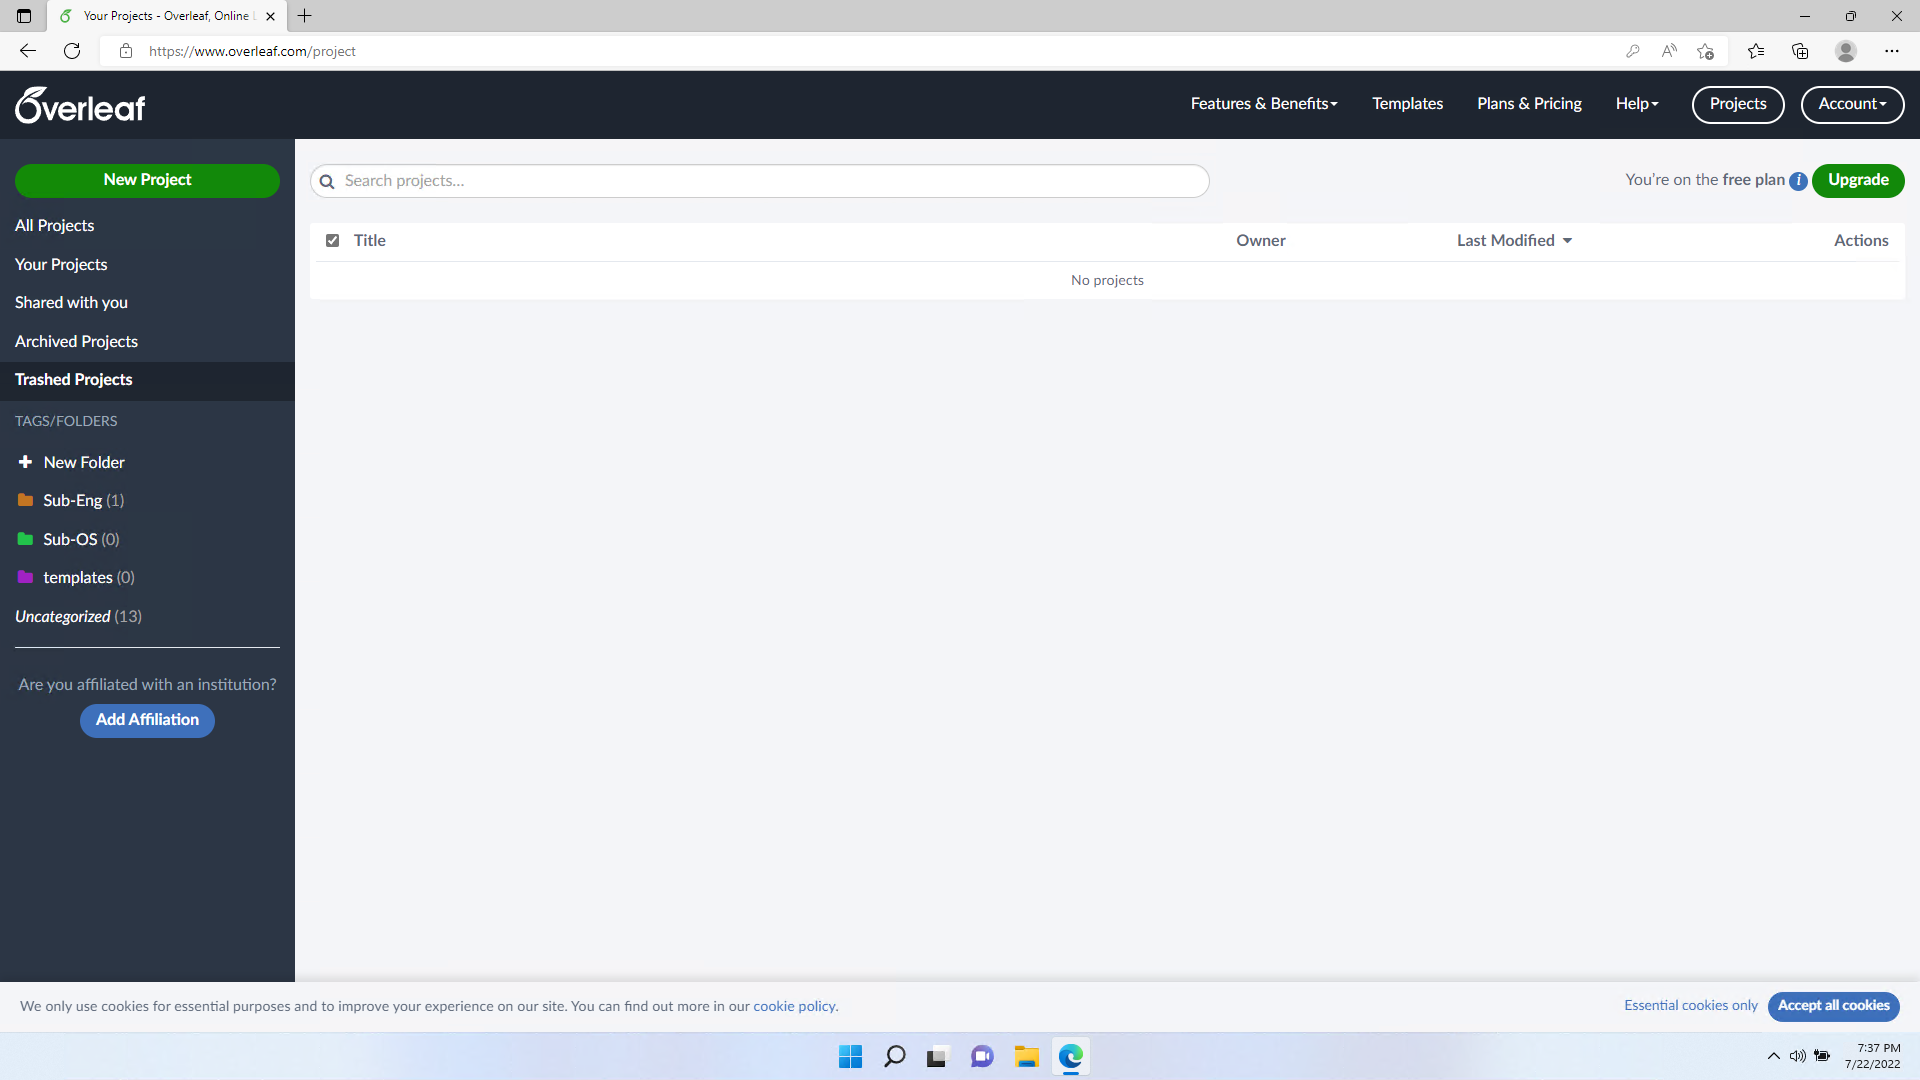
\includegraphics[width=0.9\textwidth]{figures/chapter2/overleaf-home.png}
  \caption{Overleaf项目页面}
  \label{fig:2-overlead-home}
\end{figure}

此时你需要将使用的模板下载至本地。以此项目为例,进入\url{https://github.com/Nagico/WHUExperiment},点击Download ZIP即可将模板下载到本地。该模板同时也一同放至本文档旁,可以直接使用,但仍建议从Github上下载最新版本的模板。

\begin{figure}[htb]
    \centering
    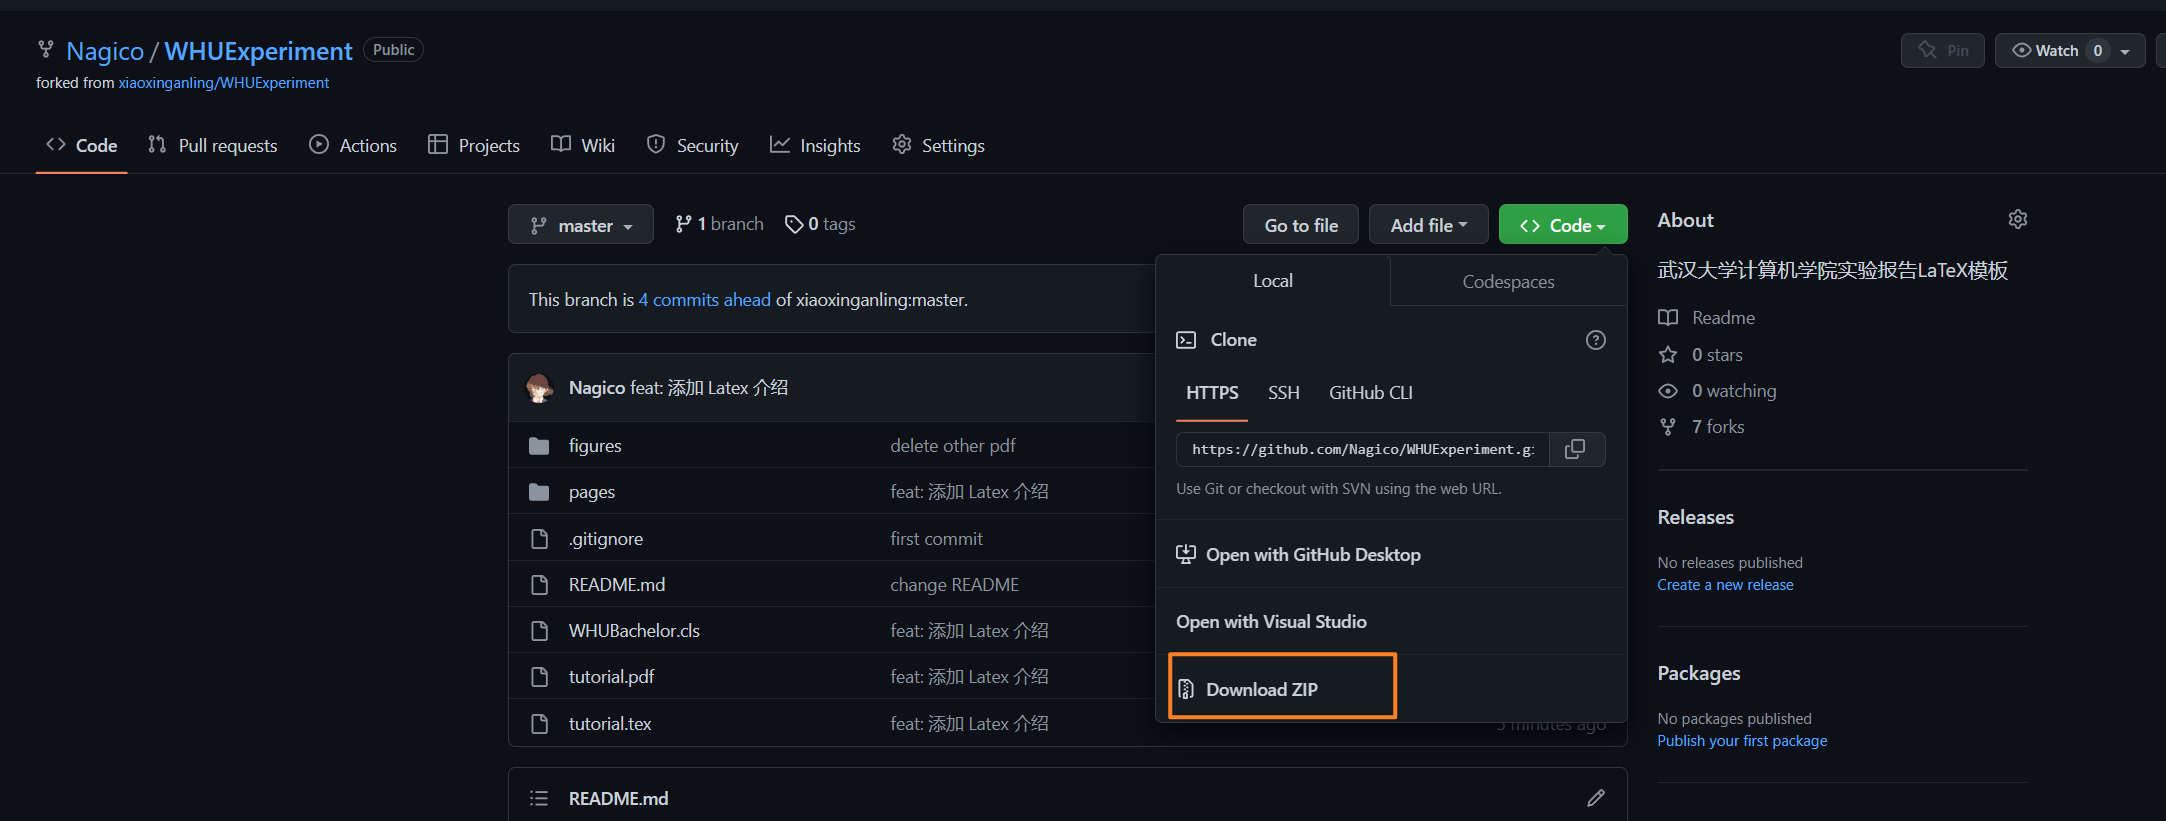
\includegraphics[width=0.95\textwidth]{figures/chapter2/download-repo.png}
    \caption{下载模板}
    \label{fig:2-github-download}
\end{figure}

在Overleaf页面点击左侧的New Project,选择Upload Project,将下载的ZIP文件上传,即可将模板导入至Overleaf。

\begin{figure}[htb]
  \centering
  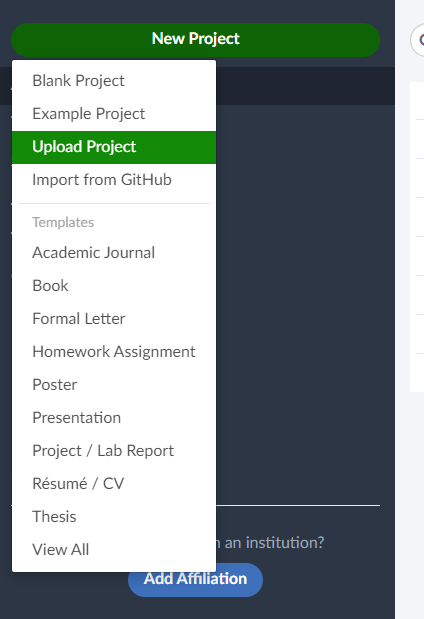
\includegraphics[width=0.3\textwidth]{figures/chapter2/upload-project.png}
  \caption{导入模板}
  \label{fig:2-upload-project}
\end{figure}

导入后会自动跳转到编辑界面,需要点击左上角的Menu进入设置界面,将Compiler修改为XeLatex以支持中文(图\ref{fig:2-compiler})。

\begin{figure}[H]
  \centering
  \begin{subfigure}{0.55\textwidth}
    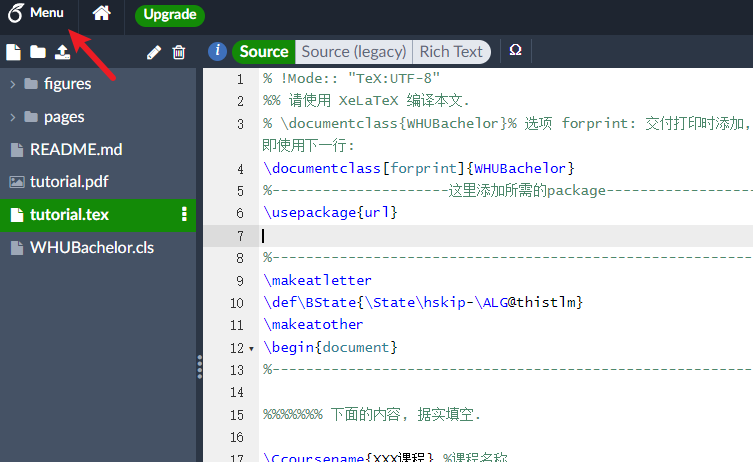
\includegraphics[width=\linewidth]{figures/chapter2/menu.png}
    \caption{Menu按钮}
    \label{fig:2-menu}
  \end{subfigure}\qquad
  \begin{subfigure}{0.3\textwidth}
    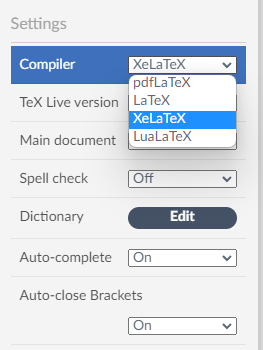
\includegraphics[width=\linewidth]{figures/chapter2/xelatex.png}
    \caption{选择Compiler}
    \label{fig:2-compiler}
  \end{subfigure}
  \caption{配置~\LaTeX~}
  \label{fig:2-latex-conf}
\end{figure}

修改成功后点击Recompile重新编辑,即可正常使用。你可以在左侧进行项目文件的管理,后续所需的图片可以在相应文件夹处右键,选择Upload上传。

\begin{figure}[htb]
  \centering
  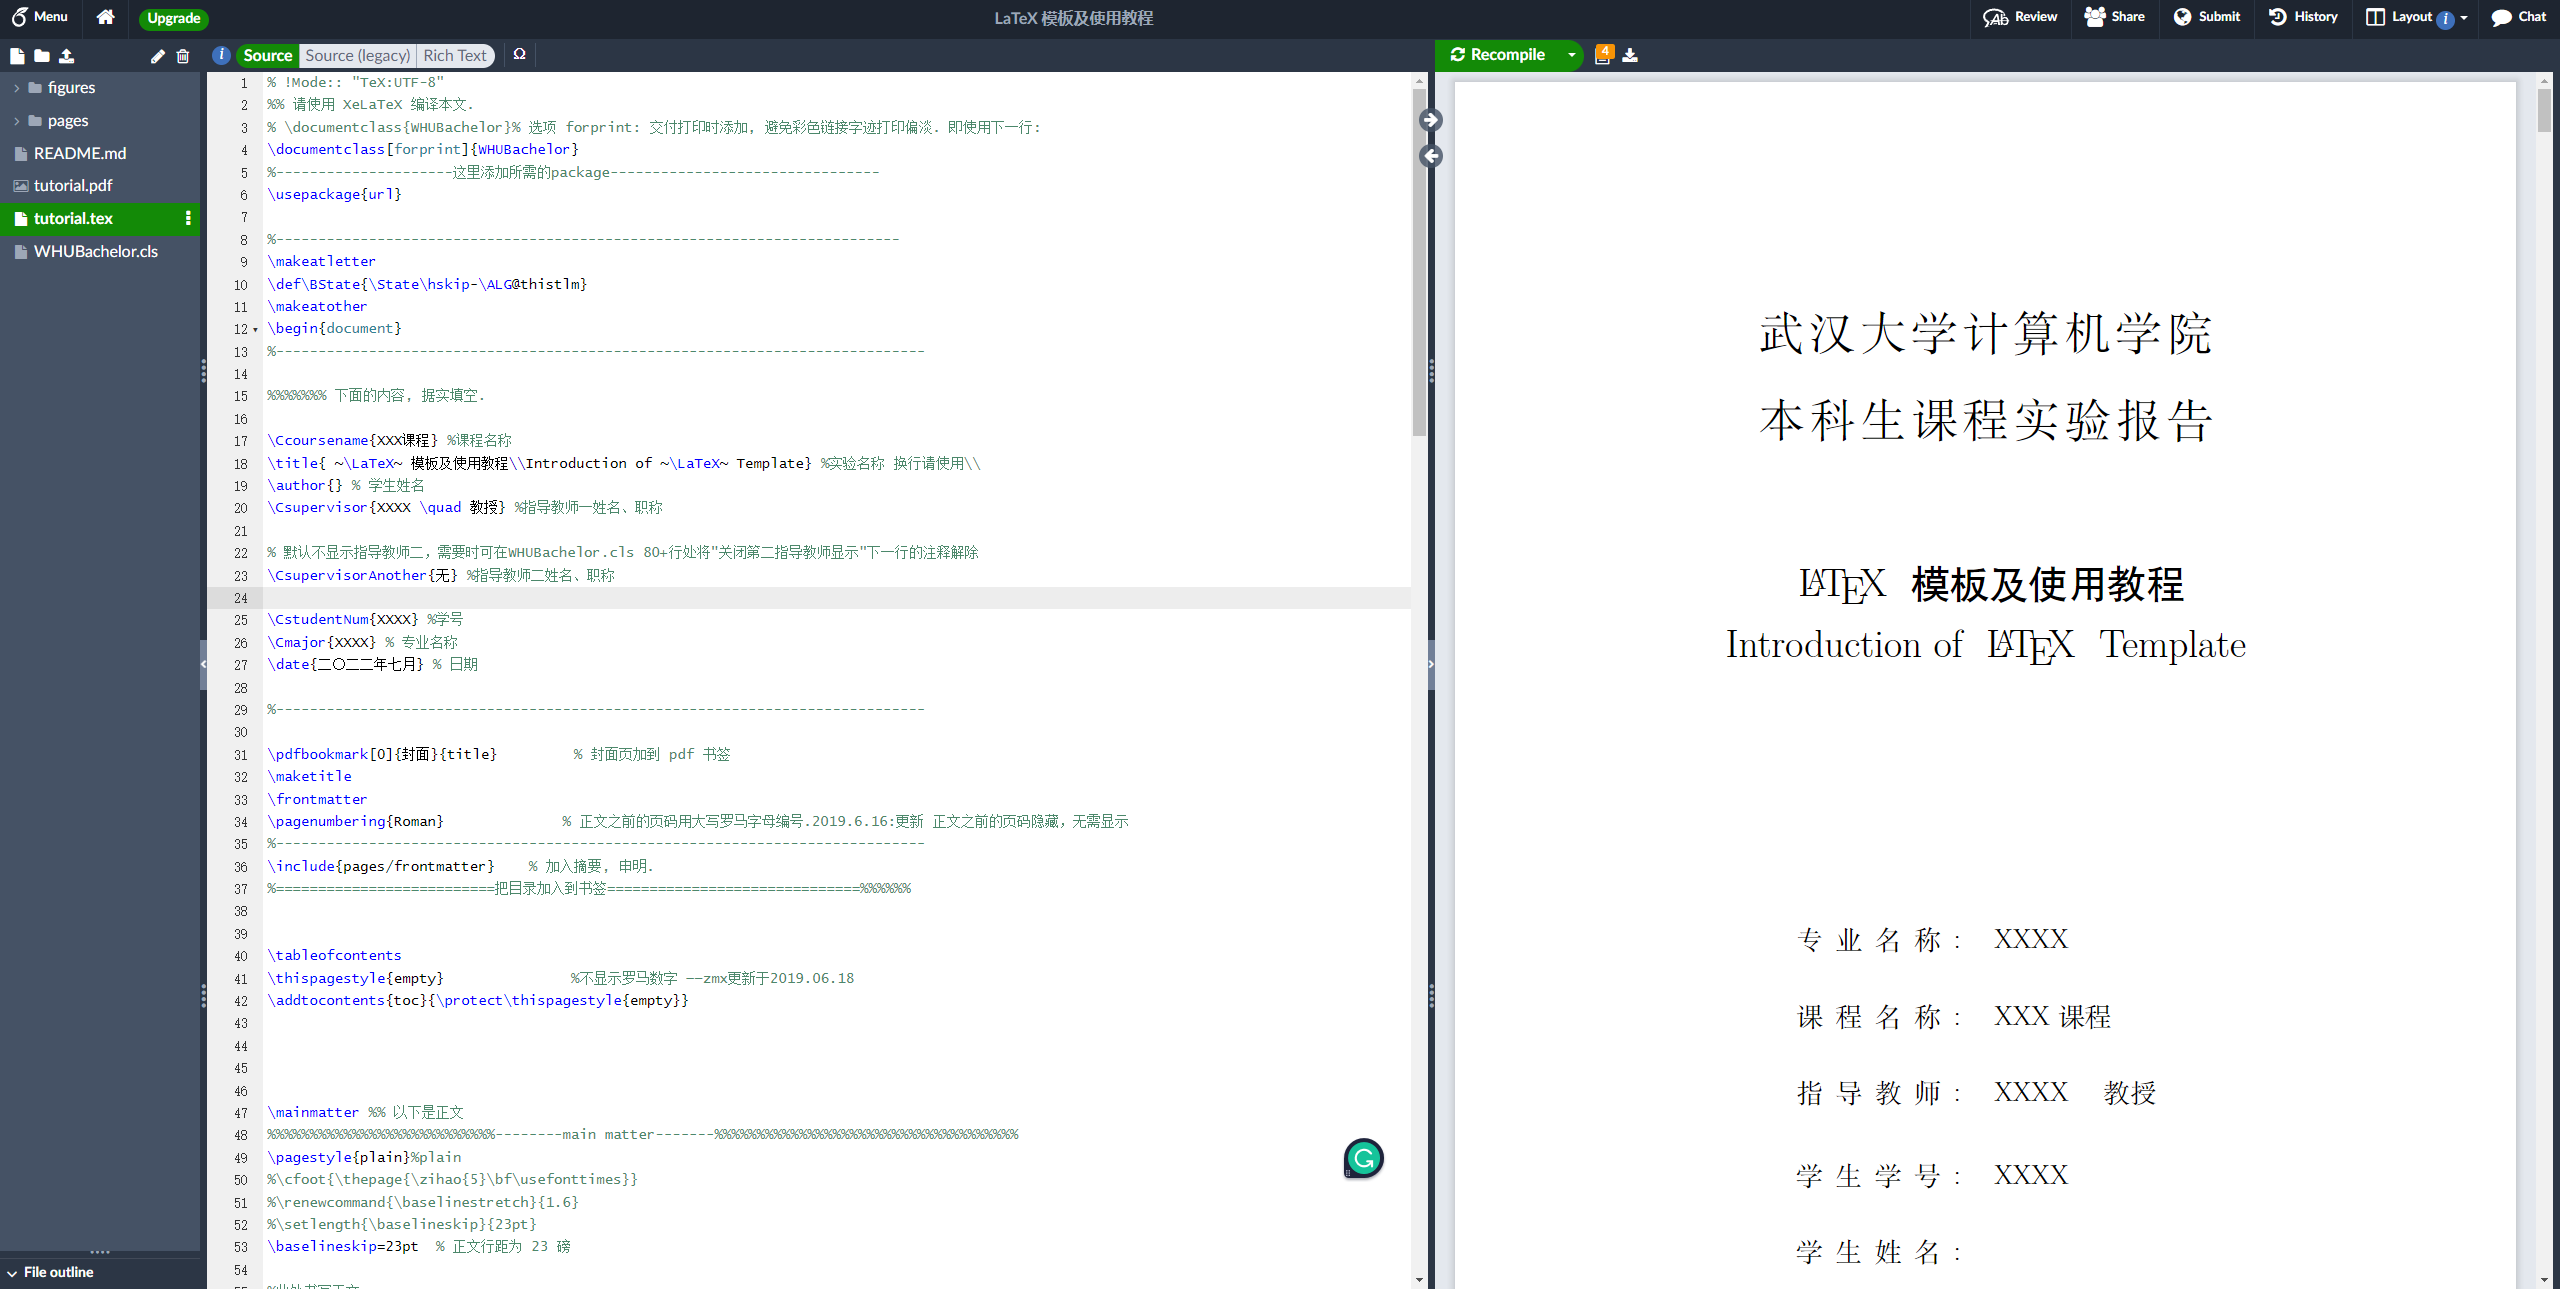
\includegraphics[width=0.95\textwidth]{figures/chapter2/overleaf-edit.png}
  \caption{Overleaf编辑页面}
  \label{fig:2-overleaf-edit}
\end{figure}

\section{本地编辑器}

\subsection{~\LaTeX~环境安装}

在清华源中下载Tex Live镜像文件:\url{https://mirrors.tuna.tsinghua.edu.cn/CTAN/systems/texlive/Images/texlive.iso},下载成功后双击挂载iso文件。


\begin{figure}[htb]
  \centering
  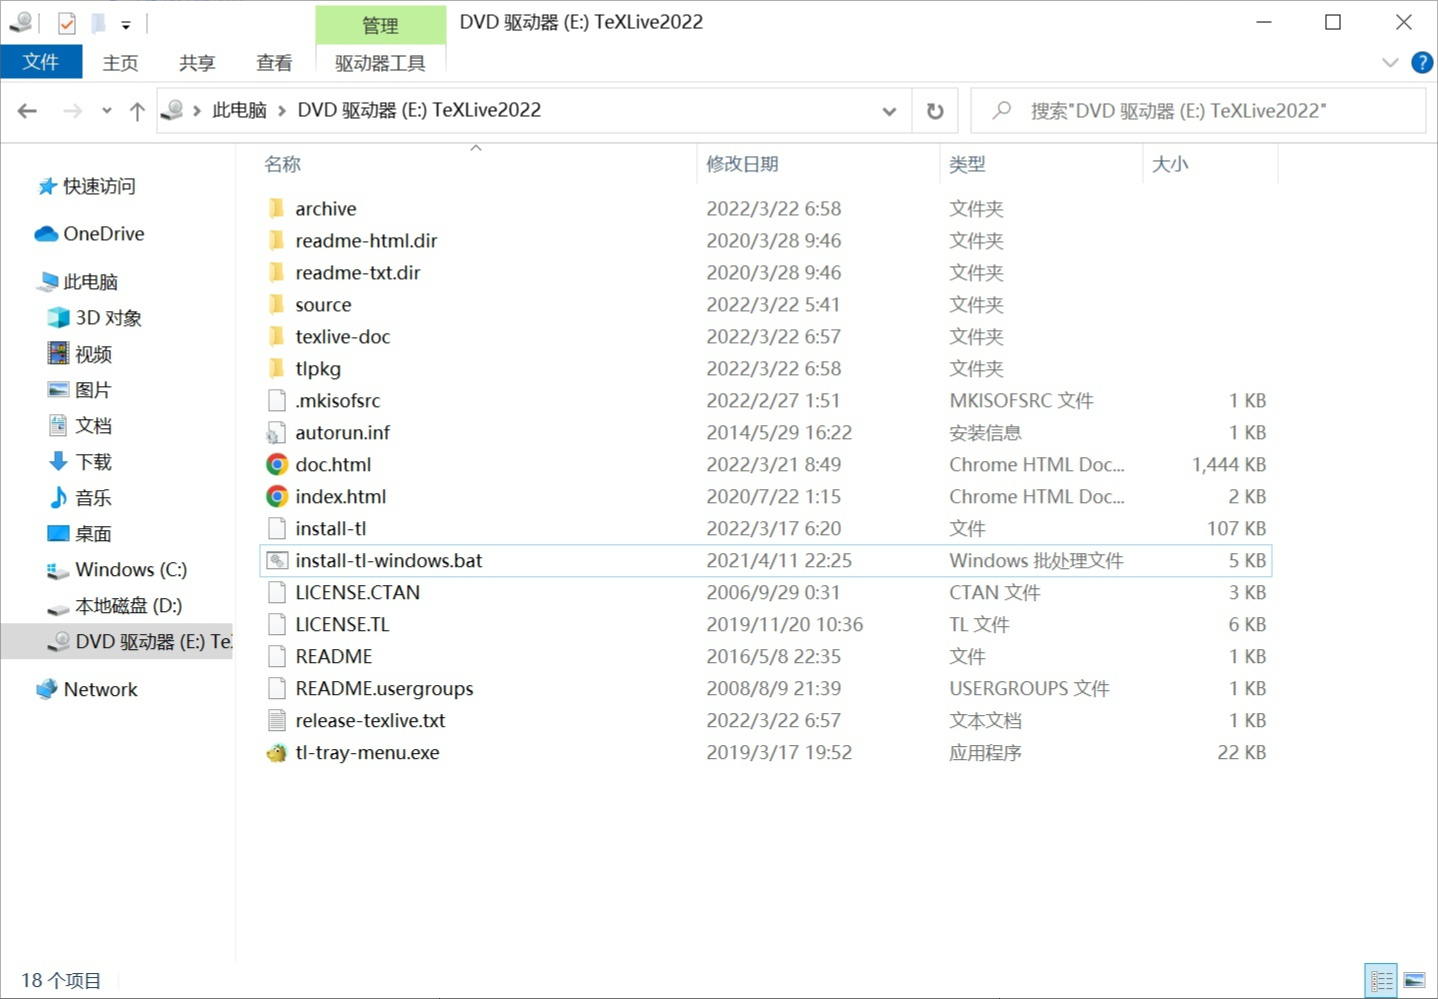
\includegraphics[width=0.95\textwidth]{figures/chapter2/texlive-iso.png}
  \caption{Tex Live镜像}
  \label{fig:2-texlive-iso}
\end{figure}

Windows下直接打开install-tl-windows.bat,Linux/Mac用户在终端下输入:

\begin{lstlisting}[language=bash]
  ./install-tl
\end{lstlisting}

使用默认配置进行安装。

\begin{figure}[htb]
  \centering
  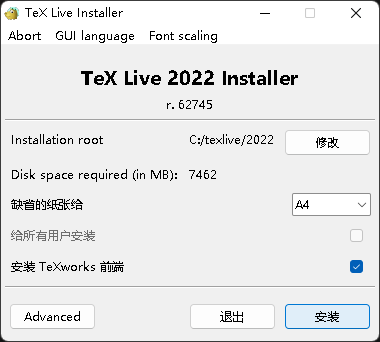
\includegraphics[width=0.4\textwidth]{figures/chapter2/texlive-install.png}
  \caption{Tex Live安装}
  \label{fig:2-texlive-install}
\end{figure}

详细安装过程和注意事项请参考:\url{https://github.com/OsbertWang/install-latex-guide-zh-cn/releases/latest/}

\subsection{VSCode配置}

Tex Live自带的编辑器不太好用,个人一般使用VSCode配合LaTeX Workshop插件。

\begin{enumerate}
  \item 点击拓展图标,打开拓展
  \item 输入"latex workshop",选择第一个LaTeX Workshop插件
  \item 点击"install"进行安装,等待安装完成(如图\ref{fig:2-plugin-install})
\end{enumerate}

\begin{figure}[H]
  \centering
  
\includegraphics[width=0.95\textwidth]{figures/chapter2/plugin-install.png}
  \caption{LaTeX Workshop插件安装}
  \label{fig:2-plugin-install}
\end{figure}

\begin{enumerate}
  \item 点击设置图标
  \item 点击设置
  \item 转到 UI 设置页面(如图\ref{fig:2-vscode-settings})
  \item 点击右上侧图标打开JSON配置文件,进入代码设置页面(如图\ref{fig:2-vscode-json})
\end{enumerate}

\begin{figure}[H]
  \centering
  \begin{subfigure}{0.45\textwidth}
    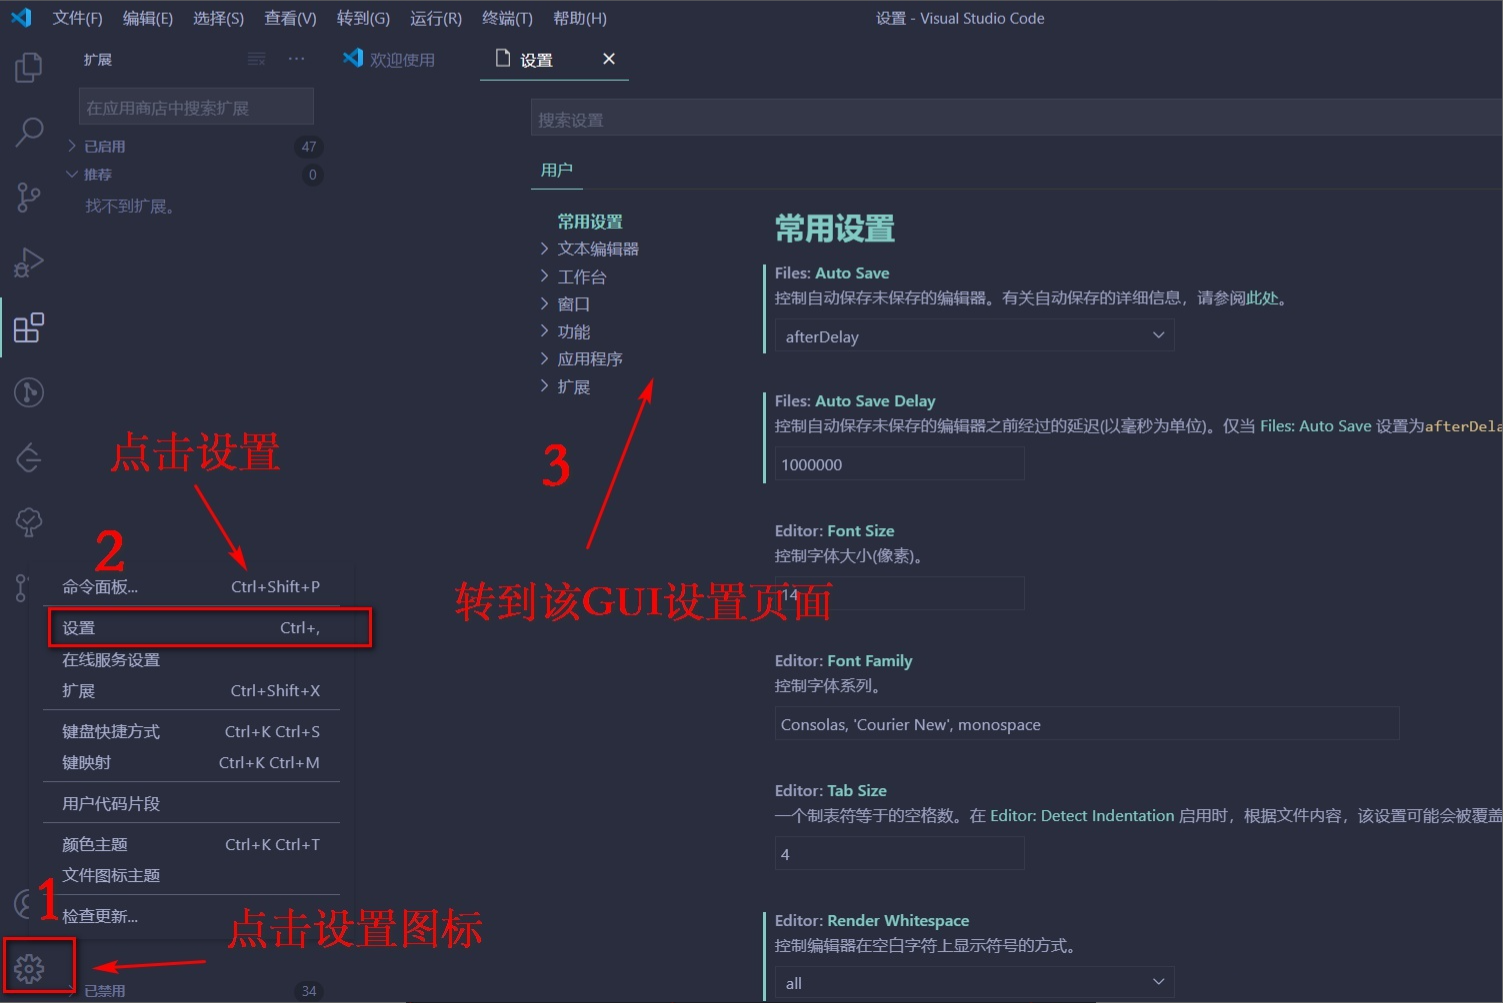
\includegraphics[width=\linewidth]{figures/chapter2/vscode-settings.png}
    \caption{UI设置界面}
    \label{fig:2-vscode-settings}
  \end{subfigure}\qquad
  \begin{subfigure}{0.45\textwidth}
    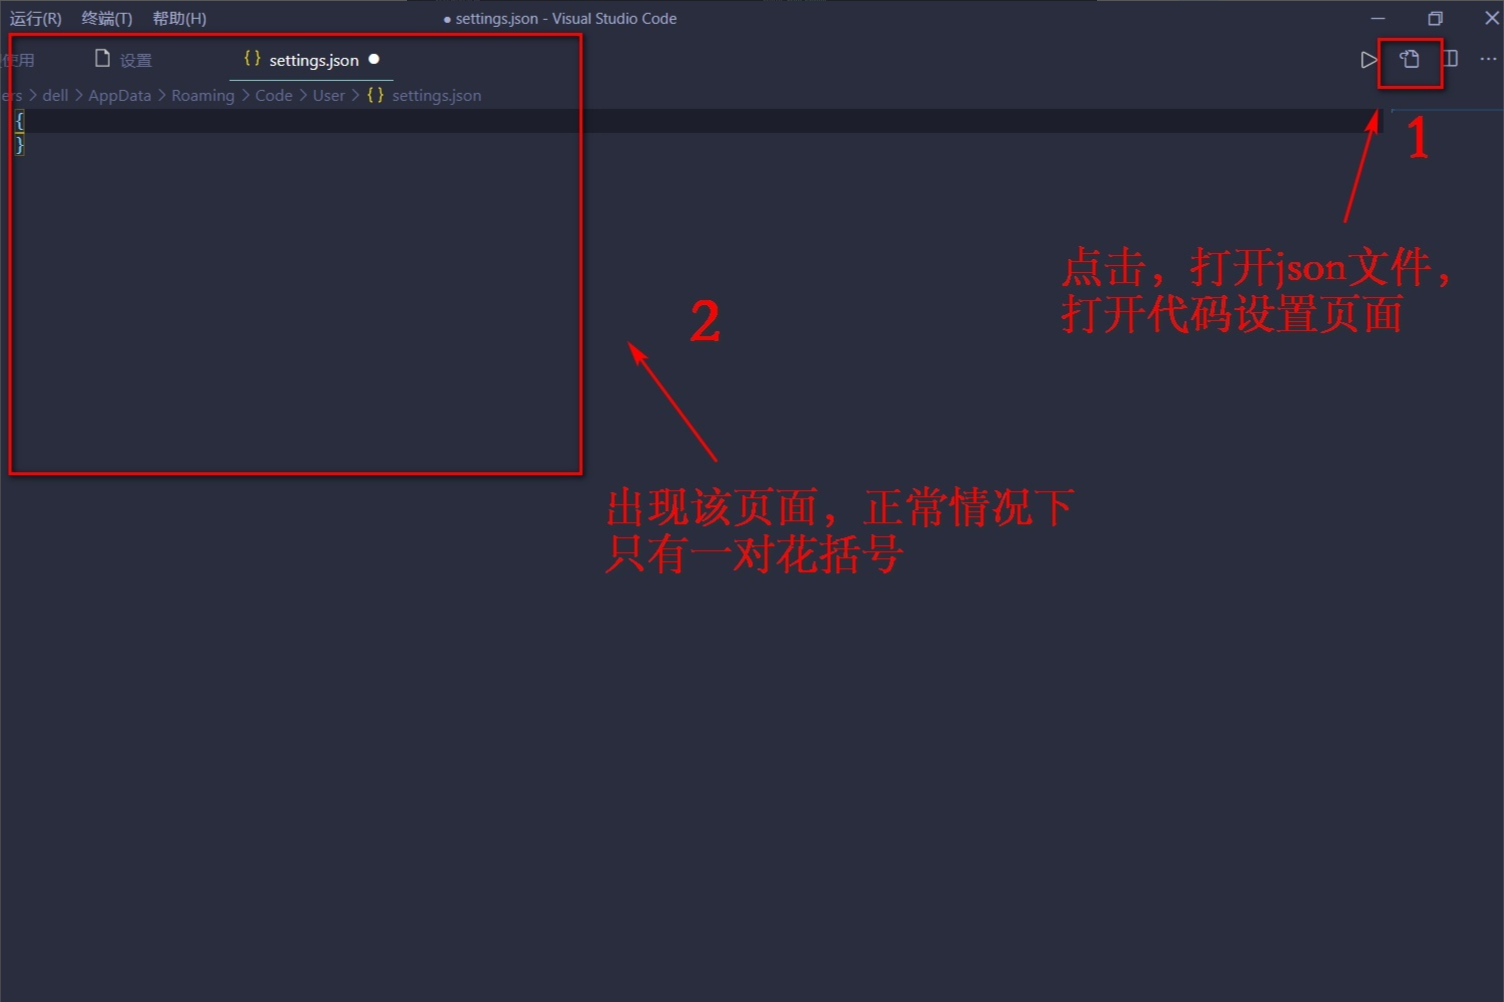
\includegraphics[width=\linewidth]{figures/chapter2/vscode-json.png}
    \caption{JSON配置文件}
    \label{fig:2-vscode-json}
  \end{subfigure}
  \caption{配置~\LaTeX~}
  \label{fig:2-vscode-conf}
\end{figure}

在JSON文件内输入以下内容:

由于PDF内代码不好复制,JSON内容请参考:\url{https://zhuanlan.zhihu.com/p/166523064}\quad \textbf{6.1 LaTeX配置代码展示}处

\begin{lstlisting}[language=json]
  {
    "latex-workshop.latex.autoBuild.run": "never",
    "latex-workshop.showContextMenu": true,
    "latex-workshop.intellisense.package.enabled": true,
    "latex-workshop.message.error.show": false,
    "latex-workshop.message.warning.show": false,
    "latex-workshop.latex.tools": [
        {
            "name": "xelatex",
            "command": "xelatex",
            "args": [
                "-synctex=1",
                "-interaction=nonstopmode",
                "-file-line-error",
                "%DOCFILE%"
            ]
        },
        {
            "name": "pdflatex",
            "command": "pdflatex",
            "args": [
                "-synctex=1",
                "-interaction=nonstopmode",
                "-file-line-error",
                "%DOCFILE%"
            ]
        },
        {
            "name": "latexmk",
            "command": "latexmk",
            "args": [
                "-synctex=1",
                "-interaction=nonstopmode",
                "-file-line-error",
                "-pdf",
                "-outdir=%OUTDIR%",
                "%DOCFILE%"
            ]
        },
        {
            "name": "bibtex",
            "command": "bibtex",
            "args": [
                "%DOCFILE%"
            ]
        }
    ],
    "latex-workshop.latex.recipes": [
        {
            "name": "XeLaTeX",
            "tools": [
                "xelatex"
            ]
        },
        {
            "name": "PDFLaTeX",
            "tools": [
                "pdflatex"
            ]
        },
        {
            "name": "BibTeX",
            "tools": [
                "bibtex"
            ]
        },
        {
            "name": "LaTeXmk",
            "tools": [
                "latexmk"
            ]
        },
        {
            "name": "xelatex -> bibtex -> xelatex*2",
            "tools": [
                "xelatex",
                "bibtex",
                "xelatex",
                "xelatex"
            ]
        },
        {
            "name": "pdflatex -> bibtex -> pdflatex*2",
            "tools": [
                "pdflatex",
                "bibtex",
                "pdflatex",
                "pdflatex"
            ]
        },
    ],
    "latex-workshop.latex.clean.fileTypes": [
        "*.aux",
        "*.bbl",
        "*.blg",
        "*.idx",
        "*.ind",
        "*.lof",
        "*.lot",
        "*.out",
        "*.toc",
        "*.acn",
        "*.acr",
        "*.alg",
        "*.glg",
        "*.glo",
        "*.gls",
        "*.ist",
        "*.fls",
        "*.log",
        "*.fdb_latexmk"
    ],
    "latex-workshop.latex.autoClean.run": "onFailed",
    "latex-workshop.latex.recipe.default": "lastUsed",
    "latex-workshop.view.pdf.internal.synctex.keybinding": "double-click"
}
\end{lstlisting}

\subsection{VSCode编译}

此时你需要将使用的模板下载至本地。以此项目为例,进入\url{https://github.com/Nagico/WHUExperiment},点击Download ZIP即可将模板下载到本地。该模板同时也一同放至本文档旁,可以直接使用,但仍建议从Github上下载最新版本的模板。

\begin{figure}[htb]
  \centering
  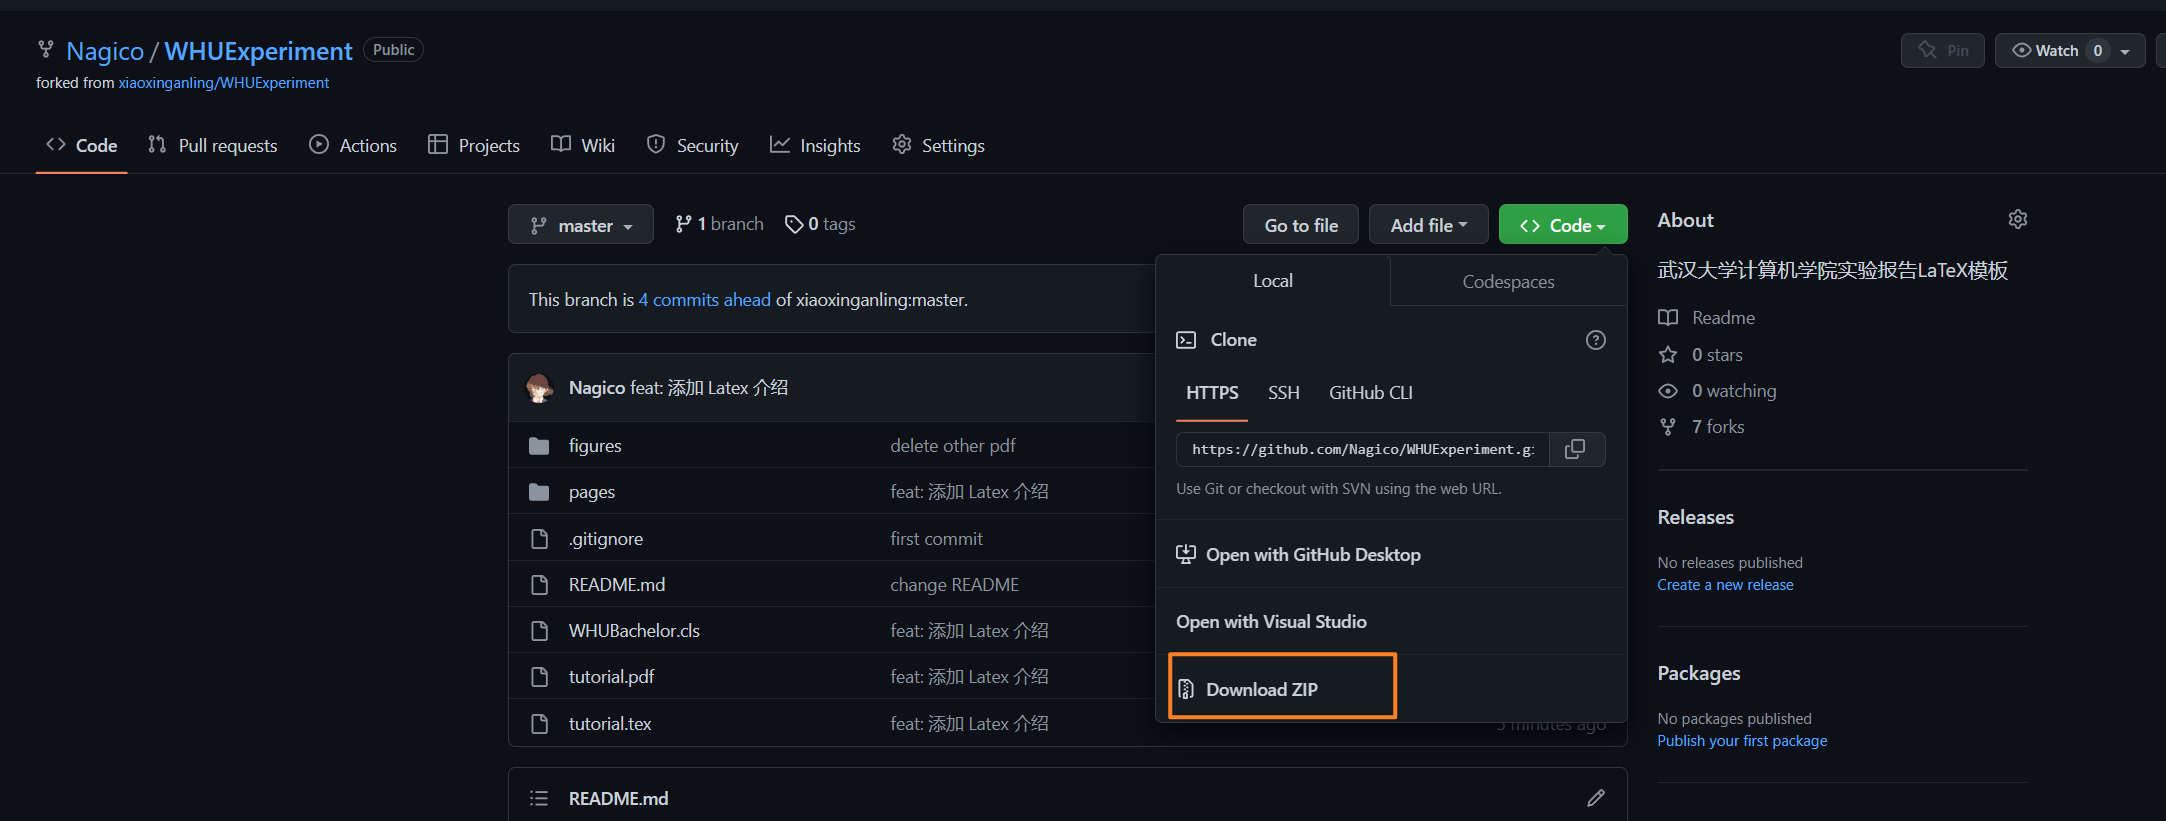
\includegraphics[width=0.95\textwidth]{figures/chapter2/download-repo.png}
  \caption{下载模板}
  \label{fig:2-github-download-2}
\end{figure}

将项目解压后用VSCode打开文件夹,点击选中 tex 文件,进行文件内容查看。

\begin{figure}[H]
  \centering
  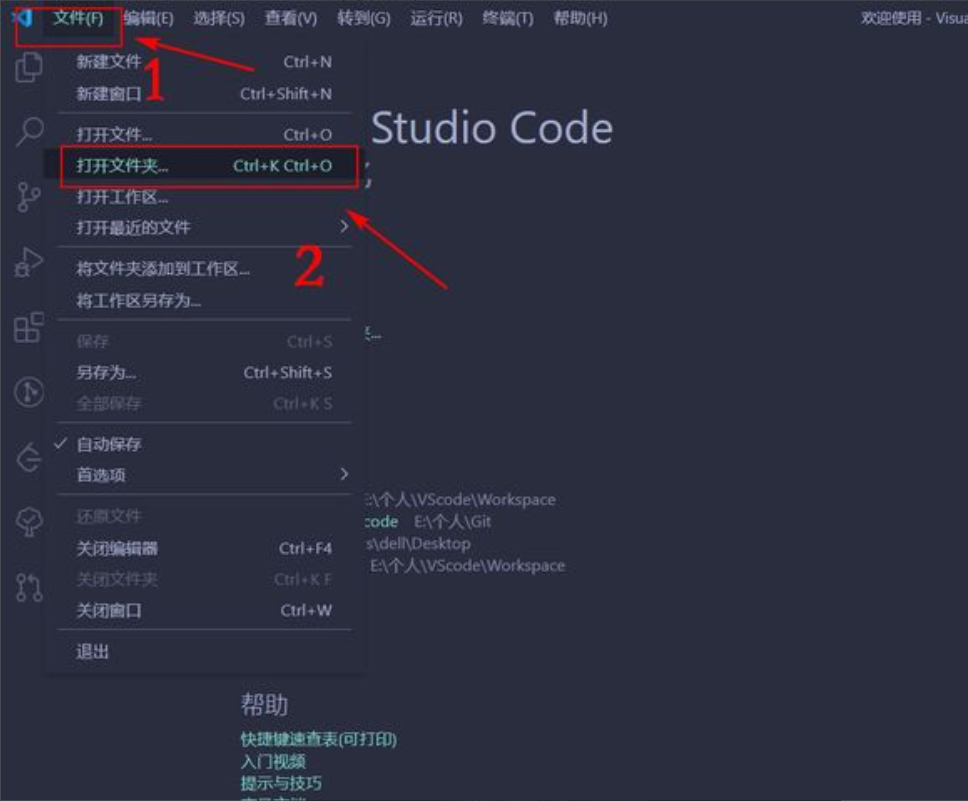
\includegraphics[width=0.9\textwidth]{figures/chapter2/vscode-open.png}
  \caption{打开项目文件夹}
  \label{fig:2-vscode-open-folder}
\end{figure}

\begin{figure}[H]
  \centering
  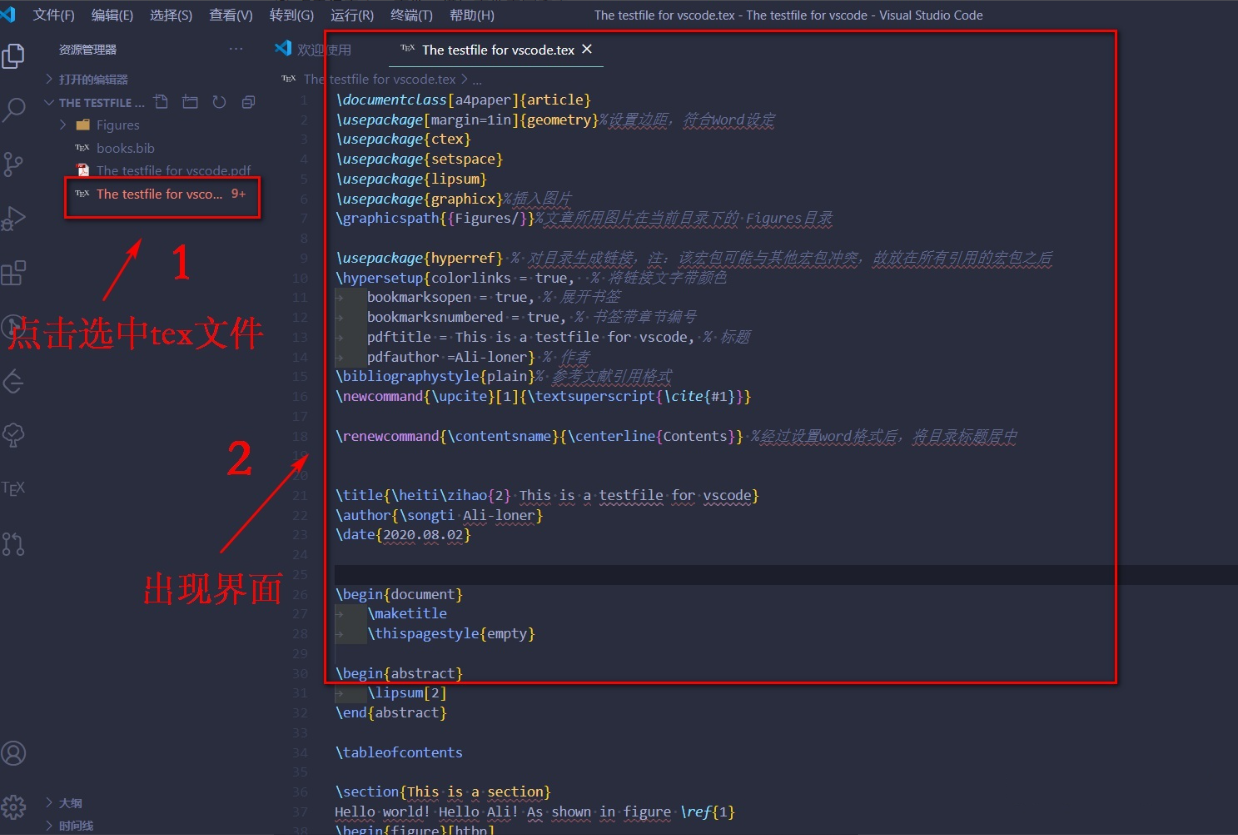
\includegraphics[width=0.9\textwidth]{figures/chapter2/vscode-openfile.png}
  \caption{打开Tex文件}
  \label{fig:2-vscode-open-file}
\end{figure}

由于项目中会涉及参考文献的引用(.bib的编译),故而选择xelatex -> bibtex -> xelatex*2编译链。

\begin{figure}[htb]
  \centering
  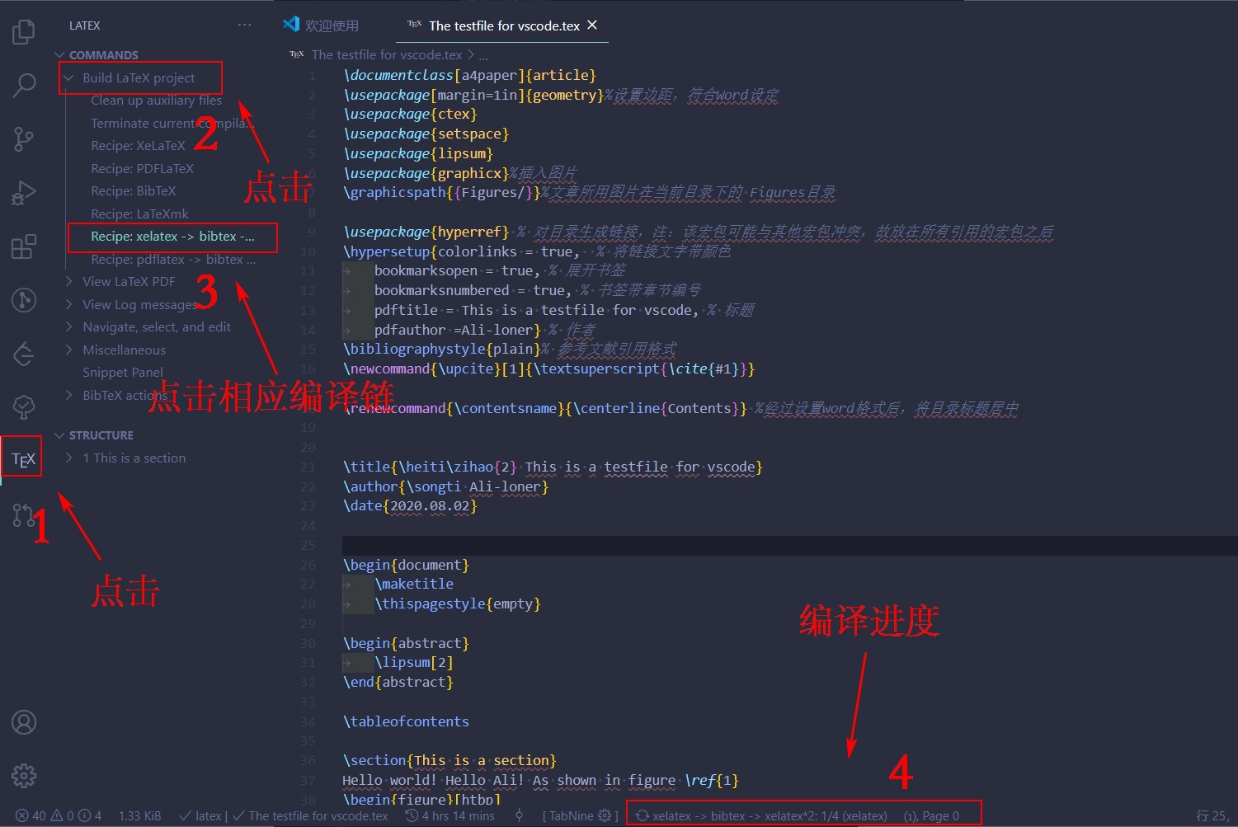
\includegraphics[width=0.8\textwidth]{figures/chapter2/vscode-compile.png}
  \caption{Tex编译}
  \label{fig:2-vscode-tex-compile}
\end{figure}

点击编辑界面的右上角图标,即可查看编译结果。

\begin{figure}[H]
  \centering
  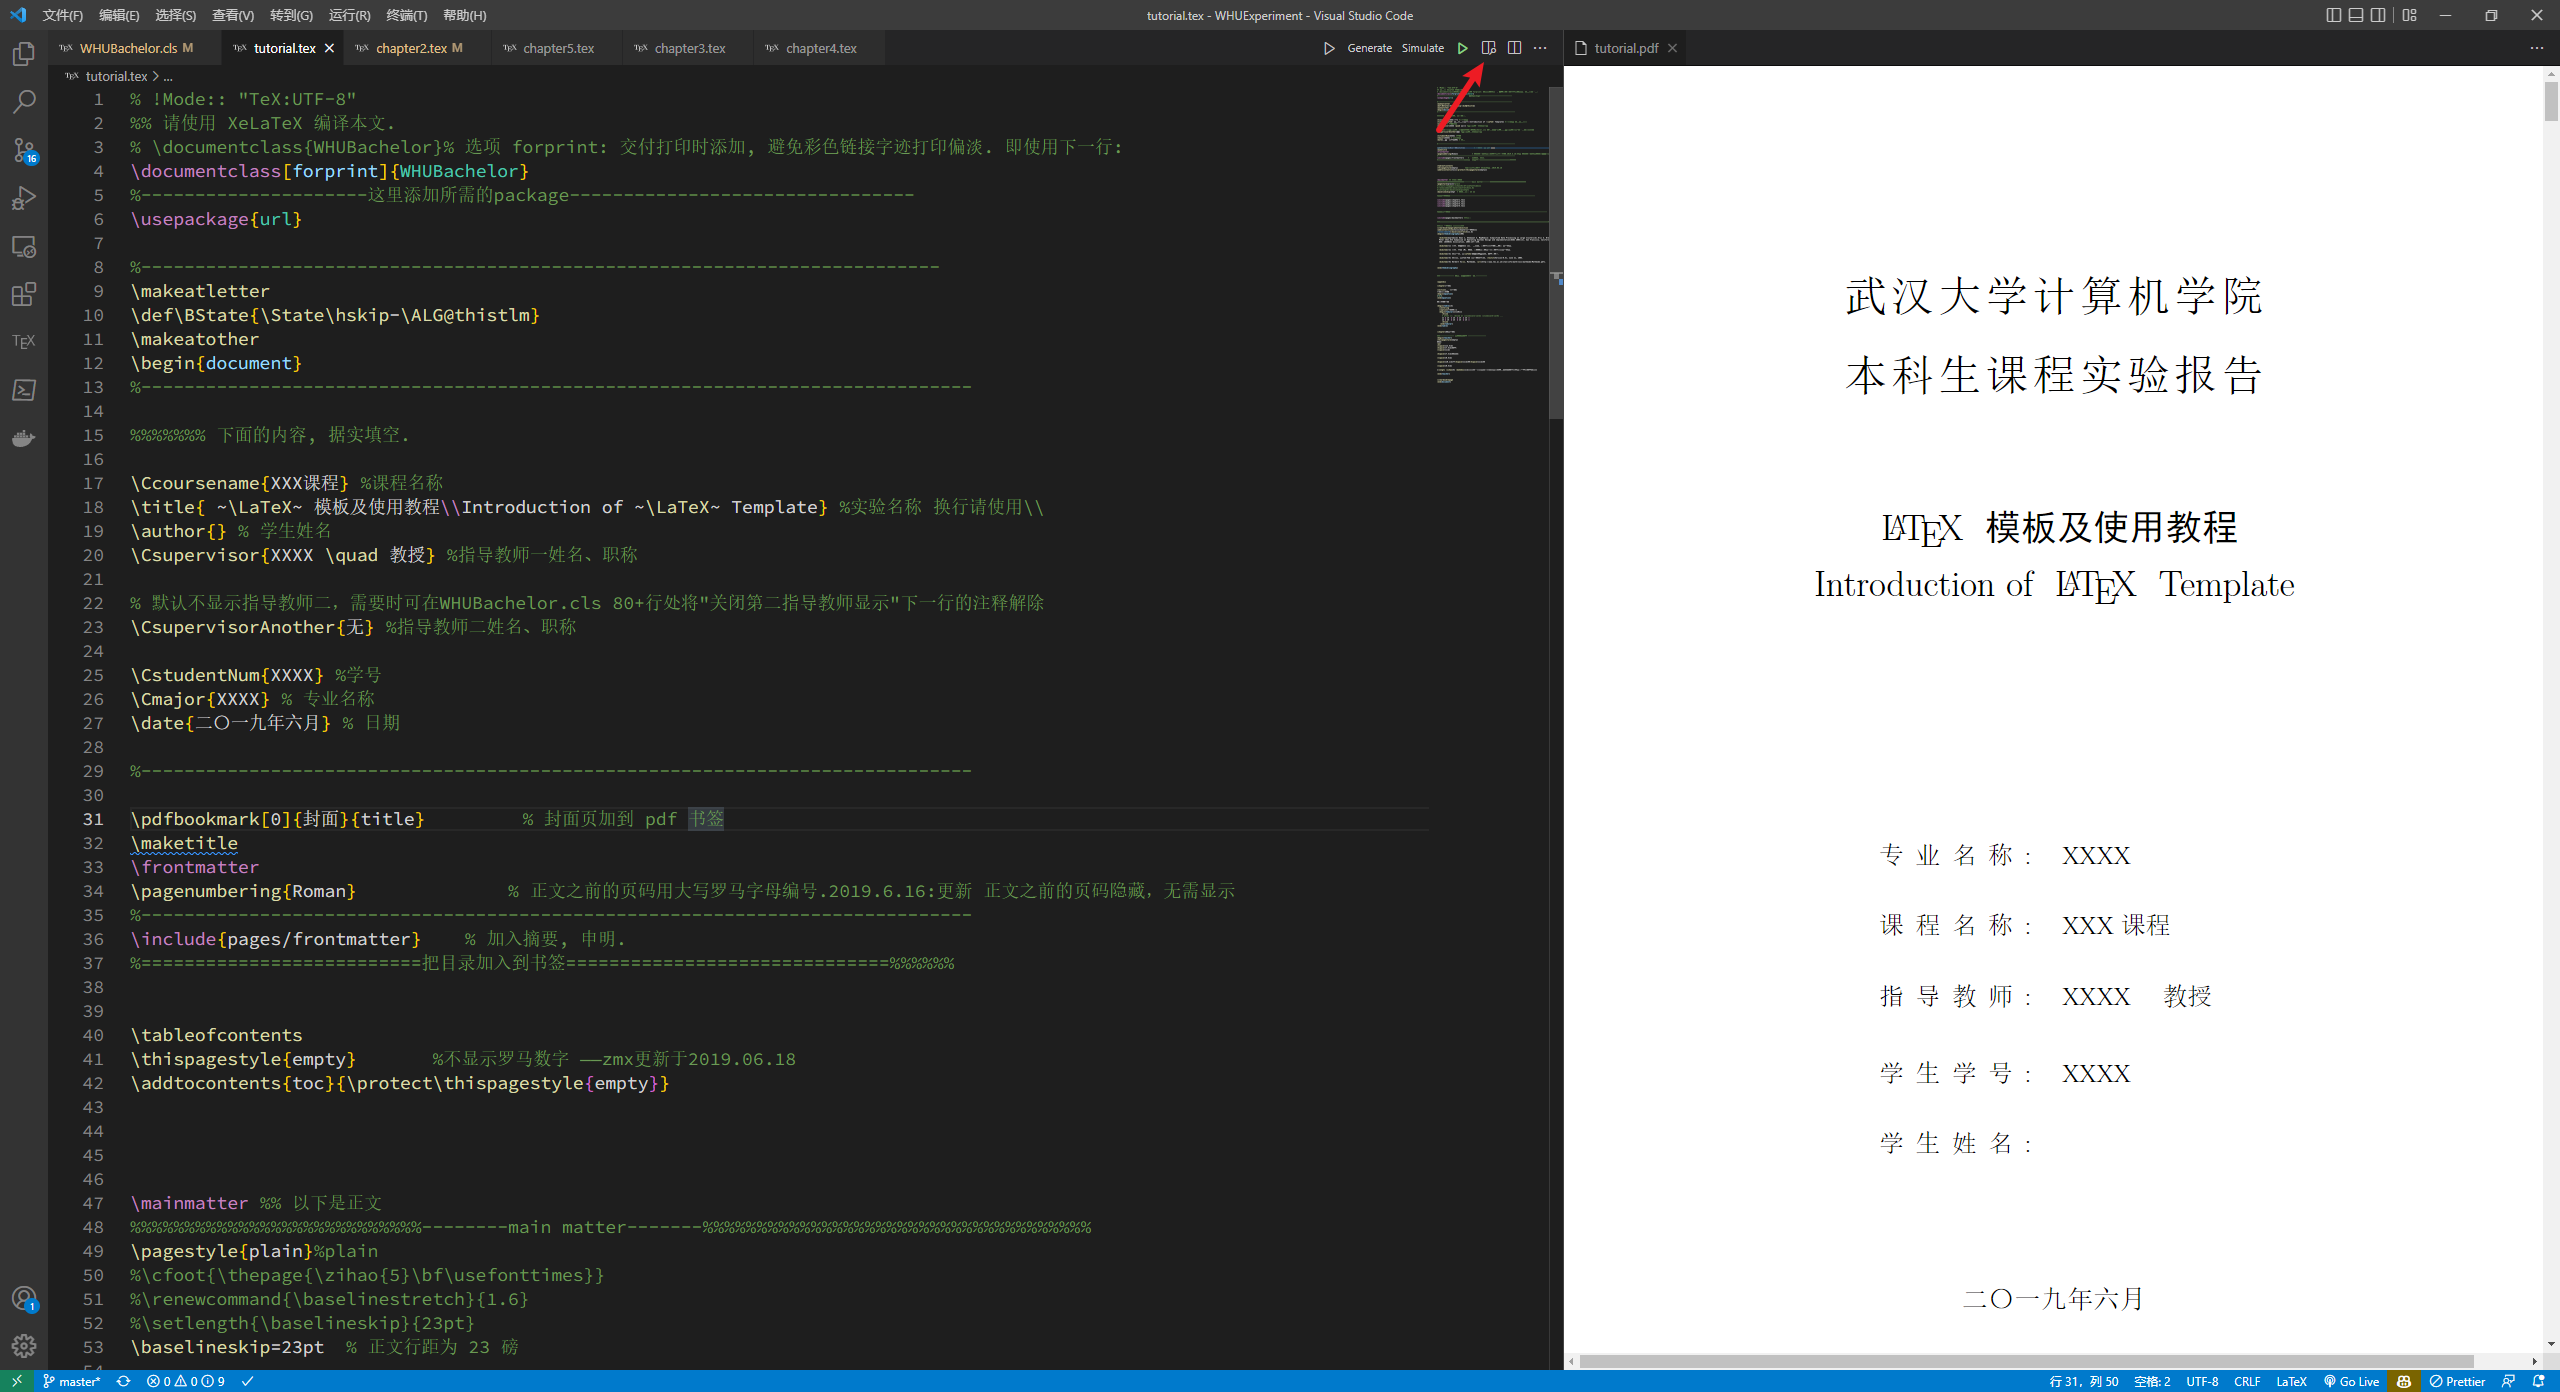
\includegraphics[width=0.95\textwidth]{figures/chapter2/vscode-edit.png}
  \caption{Tex编译结果}
  \label{fig:2-vscode-edit}
\end{figure}

更多VSCode配置可参考网上Blog,实现双向自动跳转等功能。新版VSCode、插件与以前有一定差别,最好选择2022年及以后较新的Blog学习。
\chapter{模板使用教程}
 
\section{Readme}

模板文件的结构, 如下表所示:
 \begin{table}[ht]\centering
\begin{tabular}{r|r|l}
	\hline\hline
	\multicolumn{2}{l|}{main.tex }       & 主文档. 在其中填写首页信息、正文引用、参考文献引用。             \\ \hline
                                    & chapter$x$.tex & 第$x$章节正文。             \\ \cline{2-3}
    \raisebox{1em}{pages 文件夹}   & frontmatter.tex & 郑重声明、摘要。               \\ \cline{2-3}
	 &  backmatter.tex & 实验结论.                       \\ \hline
	\multicolumn{2}{l|}{figures 文件夹}                  & 存放图片文件。                   \\ \hline
    \multicolumn{2}{l|}{ref 文件夹}                  & 存放Bib参考文献文件。                   \\ \hline
	\multicolumn{2}{l|}{WHUBachelor.cls }             & 定义文档格式的 class file。不可删除。 \\ \hline\hline
\end{tabular}
\end{table}

无需也不要改变、移动上述文档的位置。

如果不习惯用~\verb|\include{ }|~的方式加入“子文档”,当然可以把它们合并在主文档,成为一个文档。
({\kaishu 但是这样并不会给我们带来方便。})

 \section{具体使用步骤}

 \begin{description}
  \item[Step 1]  打开主文档 main.tex,填写题目、学生姓名等等信息,书写正文。
  \item[Step 2]  进入 pages 文件夹,打开 frontmatter.tex,backmatter.tex 这两个文档,
  分别填写 (1) 中文摘要,(2) 实验结论。并根据实际情况创建chapter tex文件书写正文。
  \item[Step 3]  打开主文档,在正文部分修改include的文件,注意此时不需要tex后缀名。
  \item[Step 4]  导入bib参考文献,在文档中引用。 
  \item[Step 5]  使用 XeLaTeX 编译。
\end{description}

\section{其他}

自此,~\LaTeX~安装与模板使用说明已介绍完毕。接下来的章节会以本模板支持的命令为例,讲解~\LaTeX~的使用方法。请将PDF配合Tex源码一同学习,可自行修改相关命令,查看效果。

其中 Chapter \ref{cha:latex-brief-intro}将简要的介绍~\LaTeX~使用方法,包括多级标题、字体样式、字号调节、定理与公式、图片与表格的简单使用。初次学习可以参考此章节。


 \vfill

本文档下载更新地址:\url{https://github.com/Nagico/WHUExperiment}. 使用之前,请移步查看是否有更新。
\chapter{杂七杂八的话}

\section{Readme}

模板文件的结构, 如下表所示:
 \begin{table}[ht]\centering
\begin{tabular}{r|r|l}
	\hline\hline
	\multicolumn{2}{l|}{Experiment-template.tex }       & 主文档. 在其中填写正文.             \\ \hline
	                                & frontmatter.tex & 郑重声明、摘要.               \\ \cline{2-3}
	\raisebox{1em}{includefile 文件夹} &  backmatter.tex & 实验结论.                       \\ \hline
	\multicolumn{2}{l|}{figures 文件夹}                  & 存放图片文件.                   \\ \hline
	\multicolumn{2}{l|}{WHUBachelor.cls }             & 定义文档格式的 class file. 不可删除. \\ \hline\hline
\end{tabular}
\end{table}

无需也不要改变、移动上述文档的位置.

如果不习惯用~\verb|\include{ }|~的方式加入``子文档'', 当然可以把它们合并在主文档, 成为一个文档.
({\kaishu 但是这样并不会给我们带来方便.})




 \section{字体调节}

\begin{tabular}{ll}
	\verb|\songti|   & {\songti 宋体}   \\
	\verb|\heiti|    & {\heiti 黑体}    \\
	\verb|\fangsong| & {\fangsong 仿宋} \\
	\verb|\kaishu|   & {\kaishu 楷书}
\end{tabular}


\section{字号调节}
字号命令: \verb|\zihao| \index{zihao}

\begin{tabular}{ll}
\verb|\zihao{0}| &\zihao{0}  初号字 English \\
\verb|\zihao{-0}|&\zihao{-0} 小初号 English \\
\verb|\zihao{1} |&\zihao{1}  一号字 English \\
\verb|\zihao{-1}|&\zihao{-1} 小一号 English \\
\verb|\zihao{2} |&\zihao{2}  二号字 English \\
\verb|\zihao{-2}|&\zihao{-2} 小二号 English \\
\verb|\zihao{3} |&\zihao{3}  三号字 English \\
\verb|\zihao{-3}|&\zihao{-3} 小三号 English \\
\verb|\zihao{4} |&\zihao{4}  四号字 English \\
\verb|\zihao{-4}|&\zihao{-4} 小四号 English \\
\verb|\zihao{5} |&\zihao{5}  五号字 English \\
\verb|\zihao{-5}|&\zihao{-5} 小五号 English \\
\verb|\zihao{6} |&\zihao{6}  六号字 English \\
\verb|\zihao{-6}|&\zihao{-6} 小六号 English \\
\verb|\zihao{7} |&\zihao{7}  七号字 English \\
\verb|\zihao{8} |&\zihao{8}  八号字 English \\
\end{tabular}

\section{已加入的常用宏包}

\begin{description}
%  \item[amsmath,amssymb]
  \item[cite]  参考文献引用, 得到形如 [3-7] 的样式.
  \item[color,xcolor]  支持彩色.
  \item[enumerate]  方便自由选择 enumerate 环境的编号方式. 比如

  \verb|\begin{enumerate}[(a)]| 得到形如 (a), (b), (c) 的编号.


  \verb|\begin{enumerate}[i)]| 得到形如 i), ii), iii) 的编号.

  \verb|\begin{enumerate}[\hspace{1cm}(1)]| \verb|\hspace|命令用于调整距离

\end{description}

另外要说明的是,  itemize, enumerate, description 这三种 list 环境, 已经调节了其间距和缩进,
以符合中文书写的习惯.

\section{标点符号的问题}

建议使用半角的标点符号, 后边再键入一个空格. 特别是在英文书写中要注意此问题!

双引号是由两个左单引号、两个右单引号构成的: \verb|``  ''|. 左单引号在键盘上数字~1 的左边.

但是, 无论您偏向于全角或半角, 强烈建议您使用实心的句号, 只要您书写的是自然科学的文章.
原因可能是因为, 比如使用全角句号的句子结尾处的``$x$。''容易误为数学式~$x_0$(\verb|$x_0$|)吧.



\section{引用的问题}


\subsection{参考文献的引用}

参考文献的引用, 用命令~\verb|\cite{ }|. 大括号内要填入的字串, 是自命名的文献条目名.

比如, 通常我们会说:

 {\kaishu
关于此问题, 请参见文献 \cite{r2}. 作者某某还提到了某某概念\upcite{r1}.}


上文使用的源文件为:

 {\kaishu
关于此问题, 请参见文献~\verb|\cite{r2}|. 作者某某还提到了某某概念~\verb|\upcite{r1}|.
}

其中~\verb|\upcite| 是自定义命令, 使文献引用呈现为\CJKunderdot{上标形式}.

({\heiti 注意:} {\kaishu 这里文献的引用, 有时需要以上标形式出现, 有时需要作为正文文字出现, 为什么?})

另外, 要得到形如~\cite{r1,r3,r4,r5} 的参考文献连续引用, 需要用到 cite 宏包(模板已经加入),
在正文中使用~\verb|\cite{r1,r3,r4,r5}| 的引用形式即可.
或者, 连续引用的上标形式: 使用~\verb|\upcite{r1,r2,r3}|, 得到\upcite{r1,r2,r3}.

\subsection{定理和公式的引用}

\begin{theorem}[谁发现的]\label{th-abcd}
最大的正整数是~$1$.
\end{theorem}

\begin{proof}
要找到这个最大的正整数, 我们设最大的正整数为~$x$, 则~$x \geqslant 1$, 两边同时乘以~$x$, 得到
\begin{equation}\label{eq-abc}
x^2 \geqslant x.
\end{equation}
而~$x$ 是最大的正整数, 由~\eqref{eq-abc} 式得到
\[
x^2 = x.
\]
所以
\begin{equation*}
x = 1.
\end{equation*}
\end{proof}

定理~\ref{th-abcd} 是一个重大的发现.

%%%%----- 定义等环境的举例 --------
\begin{definition}[整数]
 正整数(例如 1, 2, 3)、负整数(例如 ${−1}$, $−2$, $−3$)与零(0)合起来统称为{\heiti 整数}.
\end{definition}

\begin{remark}
  整数集合在数学上通常表示为 $\mathbf{Z}$ 或 $\mathbb{Z}$, 该记号源于德语单词 Zahlen(意为``数'')的首字母.
\end{remark}

\begin{proposition}
任意两个整数相加、相减、相乘的结果, 仍然是整数.
\end{proposition}

\begin{example}
  $1+2=3$.
\end{example}

\begin{corollary}
   在整数集合内, 相加、相减、相乘运算是封闭的.
\end{corollary}

\section{图形与表格}

支持对~eps, pdf, jpg 等等常见图形格式.

再次\colorbox{red!45}{澄清一个误会}: \LaTeX{} 支持的图形格式绝非 eps 这一种. 无需特意把图片转化为 eps.

用形如~\verb|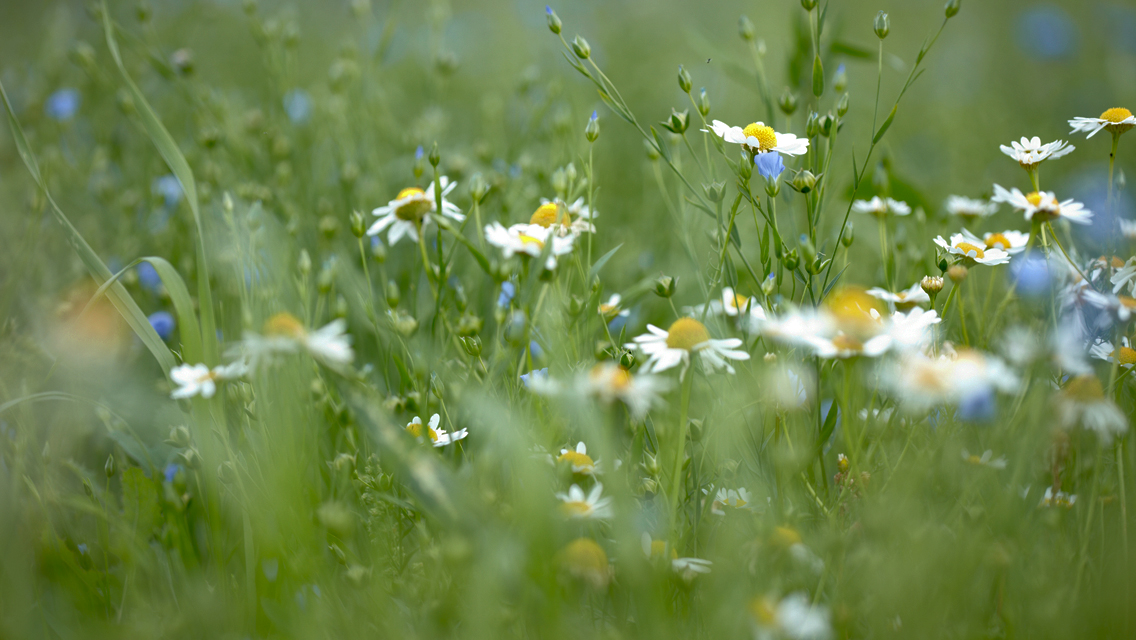
\includegraphics[width=12cm]{Daisy.jpg}| 的命令可以纳入图片.

如图~\ref{fig:1} 是一个纳入~jpg 图片的例子.

\begin{figure}[ht]
\centering
  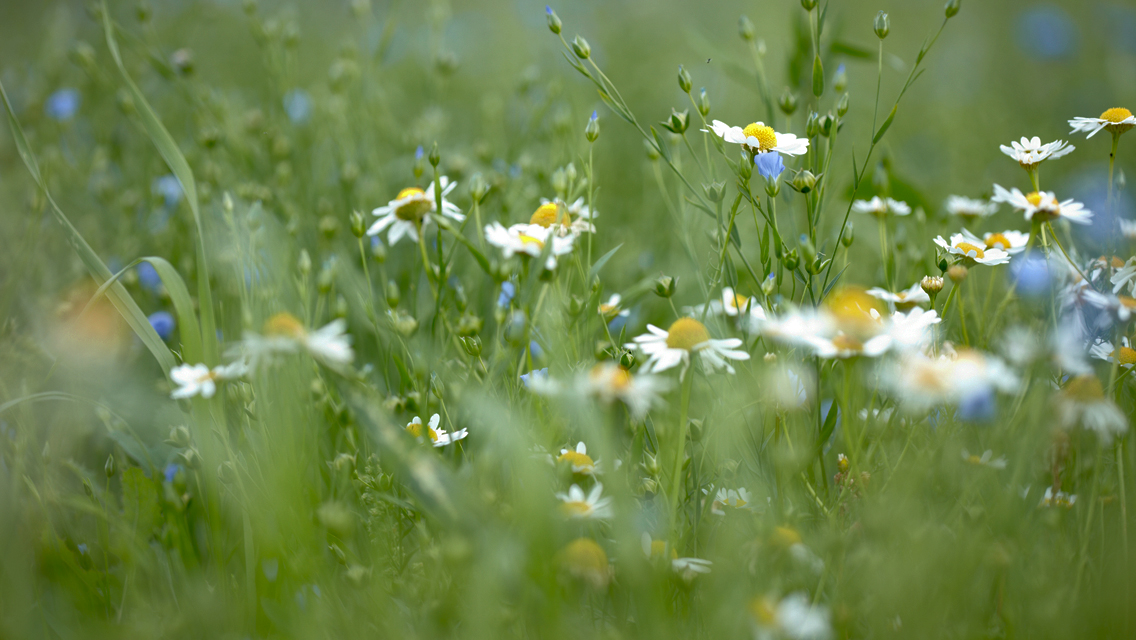
\includegraphics[width=\textwidth]{Daisy.jpg}
  \caption{一个彩色 jpg 图片的例子}
  \label{fig:1}
\end{figure}

表格问题, 建议使用``三线表'', 如表 \ref{tab:1}.

\begin{table}[ht]
\centering
\caption{一般三线表}
\label{tab:1}
    \begin{tabular}{c c c c c c c c c c c}
    \hline
    123 & 4  & 5  & 123 & 4 & 5123 & 4 & 5 & 123 & 4 & 5\\
    \hline
    67 & 890 & 13 & 123 & 4 & 5123 & 4 & 5 & 123 & 4 & 5\\
    67 & 890 & 13 & 123 & 4 & 5123 & 4 & 5 & 123 & 4 & 5\\
    67 & 890 & 13 & 123 & 4 & 5123 & 4 & 5 & 123 & 4 & 5\\
    \hline
    \end{tabular}
\end{table}


%%%%============================================================================================================%%%
\chapter{公式插图表格}
\section{公式的使用}
在文中引用公式可以这么写:\(a^2 + b^2 = c^2\)。这是勾股定理,它还可以表示为 \(c = \sqrt{a^2 + b^2}\)。还可以让公式单独一段并且加上编号:
\begin{equation}
  \sin^2{\theta} + \cos^2{\theta} = 1 \label{eq:pingfanghe}
\end{equation}
注意,公式前请不要空行。

还可以通过添加标签在正文中引用公式,如式\eqref{eq:pingfanghe}。

我们还可以轻松打出一个漂亮的矩阵:
\begin{equation}
  A =
  \begin{bmatrix}
    1  & 2  & 3  & 4  \\
    11 & 22 & 33 & 44 \\
  \end{bmatrix} \times
  \begin{bmatrix}
    22 & 24 \\
    32 & 34 \\
    42 & 44 \\
    52 & 54 \\
  \end{bmatrix}
\end{equation}

或者多行对齐的公式:
\begin{equation}
  \begin{aligned}
    f_1(x) & = (x + y)^2         \\
           & = x^2 + 2 x y + y^2
  \end{aligned}
\end{equation}

模板使用了 unicode-math 包更改数学字体。所以在使用数学字体时,尽量使用 unicode-math 包提供的 \verb|\sym| 接口,详情请阅读 unicode-math 文档。

\section{插图的使用}


\LaTeX{} 环境下可以使用常见的图片格式:JPEG、PNG、PDF 等。当然也可以使用 \LaTeX{} 直接绘制矢量图形,可以参考 pgf/ti\emph{k}z 等包中的相关内容。需要注意的是,无论采用什么方式绘制图形,首先考虑的是图片的清晰程度以及图片的可理解性,过于不清晰的图片将可能会浪费很多时间。

\begin{figure}[H]
  \centering
  
\includegraphics[width=0.3\textwidth]{whulogo.pdf}
  \caption{插图示例}
  \label{fig:whu}
\end{figure}

\begin{itemize}
  \item \verb|[htbp]| 选项分别是此处、页顶、页底、独立一页,排版时会优先满足前面的条件。比如 \verb|[htb]|,会从此处、页顶、页底以此尝试是否能成功显示。
  \item 当\verb|[htbp]|都无法满足“当前位置”放置时,可使用\verb|[H]|强制将图片置于当前位置。此时不满足排版规范,会产生较大的空白区域。
  \item \verb|[width=\textwidth]| 让图片占满整行,或 \verb|[width=2cm]| 直接设置宽度。
  \item 可以随时在文中进行引用,如图~\ref{fig:whu},建议缩放时保持图像的宽高比不变。
\end{itemize}

如果一个图由两个或两个以上分图组成时,各分图分别以(a)、(b)、(c)...... 作为图序,并须有分图题。模板使用 subcaption 宏包来处理,比如图~\ref{fig:subfig-a} 和图~\ref{fig:subfig-b}。

\begin{figure}[h]
  \centering
  \begin{subfigure}{0.2\textwidth}
    
\includegraphics[width=\linewidth]{whulogo.pdf}
    \caption{武汉大学校徽}
    \label{fig:subfig-a}
  \end{subfigure}\qquad
  \begin{subfigure}{0.7\textwidth}
    
\includegraphics[width=\linewidth]{whu.pdf}
    \caption{武汉大学}
    \label{fig:subfig-b}
  \end{subfigure}
  \caption{多个分图的示例}
  \label{fig:multi-image}
\end{figure}

\section{表格的使用}
表格的输入可能会比较麻烦,可以使用在线的工具,如 \href{https://www.tablesgenerator.com/}{Tables Generator} 能便捷地创建表格,也可以使用离线的工具,如 \href{https://ctan.org/pkg/excel2latex}{Excel2LaTeX} 支持从 Excel 表格转换成 \LaTeX{} 表格。\href{https://en.wikibooks.org/wiki/LaTeX/Tables}{LaTeX/Tables} 上及 \href{https://www.tug.org/pracjourn/2007-1/mori/mori.pdf}{Tables in LaTeX} 也有更多的示例能够参考。

\subsection{普通表格}
下面是一些普通表格的示例:

\begin{table}[H]
  \centering
  \caption{简单表格}
  \label{tab:1}
  \begin{tabular}{|l|c|r|}
    \hline
    我是 & 一只 & 普通 \\
    \hline
    的   & 表格 & 呀   \\
    \hline
  \end{tabular}
\end{table}

也可以使用 booktabs 包创建三线表。

\begin{table}[H]
  \centering
  \caption{一般三线表}
  \label{tab:2}
  \begin{tabular}{ccc}
    \toprule
    姓名 & 学号 & 性别 \\
    \midrule
    张三 & 001  & 男   \\
    李四 & 002  & 女   \\
    \bottomrule
  \end{tabular}
\end{table}

三线表中三条横线分别使用 \verb|\toprule|、\verb|\midrule| 与 \verb|\bottomrule|。若要添加 \(m\)--\(n\) 列的横线,可使用 \verb|\cmidrule{m-n}| 。

要创建占满给定宽度的表格需要使用到 tabularx 包提供的 tabularx 环境。引用表格与其它引用一样,只需要如表~\ref{tab:3}。

\begin{table}[H]
  \centering
  \caption{占满文字宽度的三线表}
  \label{tab:3}
  \begin{tabularx}{\textwidth}{CCCC}
    \toprule
    序号 & 年龄 & 身高   & 体重  \\
    \midrule
    1    & 14   & 156    & 42    \\
    2    & 16   & 158    & 45    \\
    3    & 14   & 162    & 48    \\
    4    & 15   & 163    & 50    \\
    \cmidrule{2-4} %添加2-4列的中线
    平均 & 15   & 159.75 & 46.25 \\
    \bottomrule
  \end{tabularx}
\end{table}

\subsection{跨页表格}
跨页表格常用于附录(把正文懒得放下的实验数据统统放在附录的表中)。一般使用 longtable 包提供的 longtable 环境。若要要创建占满给定宽度的跨页表格,可以使用 xltabular 包提供的 xltabular 环境,使用方法与 longtable 类似。以下是一个文字宽度的跨页表格的示例:

\begin{xltabular}{\textwidth}{CCCCCCCCC}
  \caption{文字宽度的跨页表格示例}  \\
  \toprule
  1 & 0 & 5 & 1 & 2 & 3 & 4 & 5 & 6 \\
  \midrule
  \endfirsthead

  \multicolumn{9}{l}{接上一页}      \\
  \toprule
  1 & 0 & 5 & 1 & 2 & 3 & 4 & 5 & 6 \\
  \midrule
  \endhead

  \toprule
  \multicolumn{9}{r}{转下一页}
  \endfoot

  \bottomrule
  \endlastfoot

  1 & 0 & 5 & 1 & 2 & 3 & 4 & 5 & 6 \\
  1 & 0 & 5 & 1 & 2 & 3 & 4 & 5 & 6 \\
  1 & 0 & 5 & 1 & 2 & 3 & 4 & 5 & 6 \\
  1 & 0 & 5 & 1 & 2 & 3 & 4 & 5 & 6 \\
  1 & 0 & 5 & 1 & 2 & 3 & 4 & 5 & 6 \\
  1 & 0 & 5 & 1 & 2 & 3 & 4 & 5 & 6 \\
  1 & 0 & 5 & 1 & 2 & 3 & 4 & 5 & 6 \\
  1 & 0 & 5 & 1 & 2 & 3 & 4 & 5 & 6 \\
  1 & 0 & 5 & 1 & 2 & 3 & 4 & 5 & 6 \\
  1 & 0 & 5 & 1 & 2 & 3 & 4 & 5 & 6 \\
  1 & 0 & 5 & 1 & 2 & 3 & 4 & 5 & 6 \\
  1 & 0 & 5 & 1 & 2 & 3 & 4 & 5 & 6 \\
  1 & 0 & 5 & 1 & 2 & 3 & 4 & 5 & 6 \\
  1 & 0 & 5 & 1 & 2 & 3 & 4 & 5 & 6 \\
  1 & 0 & 5 & 1 & 2 & 3 & 4 & 5 & 6 \\
  1 & 0 & 5 & 1 & 2 & 3 & 4 & 5 & 6 \\
  1 & 0 & 5 & 1 & 2 & 3 & 4 & 5 & 6 \\
  1 & 0 & 5 & 1 & 2 & 3 & 4 & 5 & 6 \\
  1 & 0 & 5 & 1 & 2 & 3 & 4 & 5 & 6 \\
  1 & 0 & 5 & 1 & 2 & 3 & 4 & 5 & 6 \\
\end{xltabular}

\section{列表的使用}
下面演示了创建有序及无序列表,如需其它样式,\href{https://www.latex-tutorial.com/tutorials/lists/}{LaTeX Lists} 上有更多的示例。

\subsection{有序列表}
这是一个计数的列表
\begin{enumerate}
  \item 第一项
        \begin{enumerate}
          \item 第一项中的第一项
          \item 第一项中的第二项
        \end{enumerate}
  \item 第二项
        \begin{enumerate}[i] %I: 大写罗马数字,i:小写罗马数字
          \item 第一项中的第一项
          \item 第一项中的第二项
        \end{enumerate}
  \item 第三项
\end{enumerate}

\subsection{不计数列表}
这是一个不计数的列表
\begin{itemize}
  \item 第一项
        \begin{itemize}
          \item 第一项中的第一项
          \item 第一项中的第二项
        \end{itemize}
  \item 第二项
  \item 第三项
\end{itemize}

\begin{table}[b]
  \caption{模板定义的数学环境}\label{tab:数学环境}
  \begin{tabularx}{\textwidth}{CCCC}
    \toprule
    theorem     & definition & lemma  & corollary \\
    定理        & 定义       & 引理   & 推论      \\
    \midrule
    proposition & example    & remark & proof     \\
    性质        & 例         & 注     & 证明      \\
    \bottomrule
  \end{tabularx}
\end{table}

\section{数学环境的使用}
模板简单定义了 8 种数学环境,具体见表~\ref{tab:数学环境},使用方法如下所示。

\begin{theorem}
  设向量 \(\vb*{a} \neq \vb*{0}\),那么向量 \(\vb*{b} \parallel \vb*{a}\) 的充分必要条件是:存在唯一的实数 \(\lambda\),使 \(\vb*{b} = \lambda \vb*{a}\)。
\end{theorem}
\begin{definition}
  这是一条定义。
\end{definition}
\begin{lemma}
  这是一条引理。
\end{lemma}
\begin{corollary}
  对数轴上任意一点 \(P\),轴上有向线段 \(\overrightarrow{OP}\) 都可唯一地表示为点 \(P\) 的坐标与轴上单位向量 \(\vb*{e}_u\) 的乘积:\(\overrightarrow{OP} = u \vb*{e}_u\)。
\end{corollary}
\begin{proposition}
  这是一条性质。
\end{proposition}
\begin{example}
  这是一条例。
\end{example}
\begin{remark}
  这是一条注。
\end{remark}
\begin{proof}
  留作练习。
\end{proof}

\section{单位}
单位的输入请使用 siunitx 包中提供的 \verb|\si| 与 \verb|\SI| 命令,可以方便地处理希腊字母以及数字与单位之间的空白。在以前,\LaTeX{} 中输入角度需要使用 \verb|$^\circ$| 的奇技淫巧,现在只需要 \verb|\ang| 命令解决问题。当然 siunitx 包中还提供了不少其他有用的命令,有需要的可以自行阅读 siunitx 文档。

示例:\SI{6.4e6}{m},\SI{9}{\micro\meter},\si{kg.m.s^{-1}},\ang{104;28;}。

\section{物理符号}
physics 宏包可以让用户更加方便、简洁地使用、输入物理符号,具体也请自行阅读 physics 文档。示例如下
\begin{equation}
  \begin{aligned}
    \int_0^{2\symup{\pi}} \abs{\sin{x}} \dd{x} & = 2 \int_0^{\symup{\pi}} \sin{x} \dd{x} \\
    & = -2 \eval{\cos{x}}_0^{\symup{\pi}}     \\
    & = 4
  \end{aligned}
\end{equation}
\chapter{引用与链接}\label{cha:ref}

\section{引用文中小节}\label{sec:ref}
如引用小节~\ref{sec:ref}

\section{引用参考文献}
这是一个参考文献引用的范例:“\cite{江泽民1989能源发展趋势及主要节能措施}提出……”。还可以引用多个文献:“\cite{kuhn2004man,江泽民2008新时期我国信息技术产业的发展,江泽民1989能源发展趋势及主要节能措施}提出……”。

参考文献根据学校推荐的格式采用abbrv样式的参考文献引用,可以在main.tex中找到bibliographystyle进行修改。以下的引用方式在abbrv时会产生错误,可修改为plainnat即可正常编译。

不同的引用方法:“\citet{江泽民1989能源发展趋势及主要节能措施}”“\citep{江泽民2008新时期我国信息技术产业的发展}”更多引用命令请参阅 natbib 文档或 biblatex 文档。\nocite{*}

文献引用需要配合 BibTeX 使用,很多工具可以直接生成 BibTeX 文件(如 Zotero、EndNote、NoteExpress、百度学术、谷歌学术等),此处不作介绍。

\section{链接相关}
模板使用了 hyperref 包处理相关链接,使用 \verb|\href| 可以生成超链接,默认不显示链接颜色。如果需要输出网址,可以使用 \verb|\url| 命令,示例:\url{https://github.com}。
\chapter{其它格式}
\section{代码}
\subsection{原始代码}
朴实的代码块:

使用 verbatim 环境可以得到如下原样的输出。
\begin{verbatim}
print("Hello world!")
\end{verbatim}

使用 listings 包提供的 lstlisting 环境可以对代码进行进一步的格式化,minted 包所提供的 minted 环境还可以对代码进行高亮。更多定制功能请自行参照文档配置。

\begin{lstlisting}[language=c]
    printf("Hello world!");
\end{lstlisting}

\subsection{算法描述/伪代码}
参考 \href{https://en.wikibooks.org/wiki/LaTeX/Algorithms}{Algorithms} 与 algorithm2e 文档,给出一个简单的示例,见算法 \ref{alg:alg1}。

\begin{algorithm}[H]
  \SetAlgoLined
  \KwData{this text}
  \KwResult{how to write algorithm with \LaTeXe}
  initialization\;
  \While{not at end of this document}{
    read current\;
    \eIf{understand}{
      go to next section\;
      current section becomes this one\;
    }{
      go back to the beginning of current section\;
    }
  }
  \caption{如何写算法}\label{alg:alg1}
\end{algorithm}

\section{绘图}
关于使用 \LaTeX{} 绘图的更多例子,请参考 \href{https://www.overleaf.com/learn/latex/Pgfplots_package}{Pgfplots package}。一般建议使用如 Photoshop、PowerPoint 等制图,再转换成 PDF 等格式插入。

\section{写在最后}
工具不重要,对工具的合理运用才重要。希望本模板对大家的论文写作有所帮助。



%此处结束正文-------------------------------------------------------------------------------------------------


% !Mode:: "TeX:UTF-8"
%%%%%%%%%%%%%%%%%%%%%%%%%%%%-------结论--------%%%%%%%%%%%%%%%%%%%%%%%%%%%%%%%%

\acknowledgement
\addcontentsline{toc}{chapter}{结论}
%\linespread{1.5}

这里写本次实验的结论。

% 这里写本次实验的结论
















 %%%结论

%%%============================================================================================================%%%

%%%=== 参考文献 ========%%%
\cleardoublepage\phantomsection

\bibliographystyle{abbrv}        % 参考文献样式,  plain,unsrt,alpha,abbrv,chinesebst 等等
\bibliography{ref/refs.bib}



%%%-------------- 附录. 不需要可以删除.-----------


\appendix

\chapter{测试}

\section{第一个测试}
测试公式编号
\begin{equation}
1+1=2.
\end{equation}

表格编号测试

\begin{table}[h]
  \centering
  \caption{测试表格}
  \begin{tabular}{*{20}c}
     \hline
     % after \\: \hline or \cline{col1-col2} \cline{col3-col4} ...
     11 & 13  & 13  & 13  & 13 \\
     12 & 14  & 13  & 13  & 13 \\
     \hline
   \end{tabular}
\end{table}


\chapter{附录测试}

%%%-------------- 教师评语评分 ------------------
\begin{teacher}
\thispagestyle{empty}
评语: 
\par
\vspace*{12.5cm}
\hspace*{7.5cm}评分: 
\vspace*{1cm}

\hspace*{7.3cm}评阅人:

\vspace*{0.5cm}

\hspace*{10.1cm}年\hspace*{1cm}月\hspace*{1cm}日

\vspace*{0.5cm}

{\songti \zihao{4} \makebox[1cm][s]{(备注:对该实验报告给予优点和不足的评价,并给出百分制评分。)}}

\end{teacher}


\cleardoublepage
\end{document}





